\documentclass{zjusct-beamer/zjusctbeamer}

% Metadata
\title{A First Look at the CPU Parallel Programming Framework}
\subtitle{PM - C++ Concurrency in Action}
\author[bowling233]{Baolin Zhu (@bowling233)}
\date{\today}
\institute[ZJUSCT]{Zhejiang University Supercomputing Team}
\copyleftnotice{CC-BY 4.0}{}

\hypersetup{
    pdftitle={\title},
    pdfpagemode=FullScreen,
}

\setminted{
    fontsize=\tiny % 设置代码和行号的字体大小
}

\begin{document}

% Set Mono and Emoji font
\setmonofont{DejaVu Sans Mono}
\setemojifont{TwemojiMozilla}

\maketitle

% Outline (Table of Contents)
%\cutoc

% Slide 正文均使用英文
\section{Introduction}

% 我的简介
\begin{frame}[fragile]{\emoji{bust-in-silhouette} Biography}
	\begin{center}
		\begin{itemize}
			\item \textbf{Baolin Zhu} (\emoji{bowling} @bowling233)
			\item (with Eric) Leader of ZJUSCT
			\item \textbf{Research Interests}: Arch/OS, Three Pillars (Compute, Network and Storage)
		\end{itemize}
		\begin{tikzpicture}
			% Timeline base line
			\draw[thick, gray] (0,0) -- (10.5,0);

			% Node 0: CKC AGC
			\fill[blue] (1.5, 0) circle (0.1);
			\draw[gray] (1.5, 0) -- (1.5, 0.5);
			\node at (1.5, 1) {
\includegraphics[width=0.8cm]{day8_pm/img/bio-ckcagc}};
			\node[font=\bfseries\small] at (1.5, 2) {CKC AGC};
			\node[font=\footnotesize, gray] at (1.5, -0.5) {Freshman};

			% Node 1: ZJUSCT
			\fill[blue] (4.0, 0) circle (0.1);
			\draw[gray] (4.0, 0) -- (4, 0.5);
			\node at (4.0, 1) {
\includegraphics[width=0.8cm]{day8_pm/img/bio-zjusct}};
			\node[font=\bfseries\small] at (4.0, 2) {ZJUSCT};
			\node[font=\footnotesize, gray] at (4.0, -0.5) {Sophomore};

			% Node 2: RC4ML Lab
			\fill[blue] (6.5, 0) circle (0.1);
			\draw[gray] (6.5, 0) -- (6.5, 0.5);
			\node at (6.5, 1) {
\includegraphics[width=0.8cm]{day8_pm/img/bio-rc4ml}};
			\node[font=\bfseries\small] at (6.5, 2) {RC4ML Lab};
			\node[font=\footnotesize, gray] at (6.5, -0.5) {Junior};

			% Node 3: Tencent
			\fill[blue] (9.0, 0) circle (0.1);
			\draw[gray] (9.0, 0) -- (9.0, 0.5);
			\node at (9.0, 1) {
\includegraphics[width=0.8cm]{day8_pm/img/bio-csig}};
			\node[font=\bfseries\small] at (9.0, 2) {Tencent CSIG};
			\node[font=\footnotesize, gray] at (9.0, -0.5) {Junior};

		\end{tikzpicture}
	\end{center}
\end{frame}

% 为什么学习 C++ 并行编程:减轻心智负担
\begin{frame}[fragile]{\emoji{question} Why C++ Concurrency?}
	Reducing cognitive overhead for \textbf{application-level} (rather than systems-level) programming.
	\begin{itemize}
		\item Object-Oriented Programming (OOP) \& Encapsulation
		\item Resource Management \& RAII: Smart pointers
		\item Templates \& Generic Programming
		\item Standard Template Library (STL) \& Abstractions
		\item Safer Concurrency Models
		\item Enhanced Type Safety \& Expressiveness: References, Function Overloading, and Lambdas
	\end{itemize}
\end{frame}

% 本节课的参考教材
\begin{frame}[fragile]{\emoji{books} Textbook}

	\begin{columns}
		\begin{column}{0.4\textwidth}
			\begin{center}
				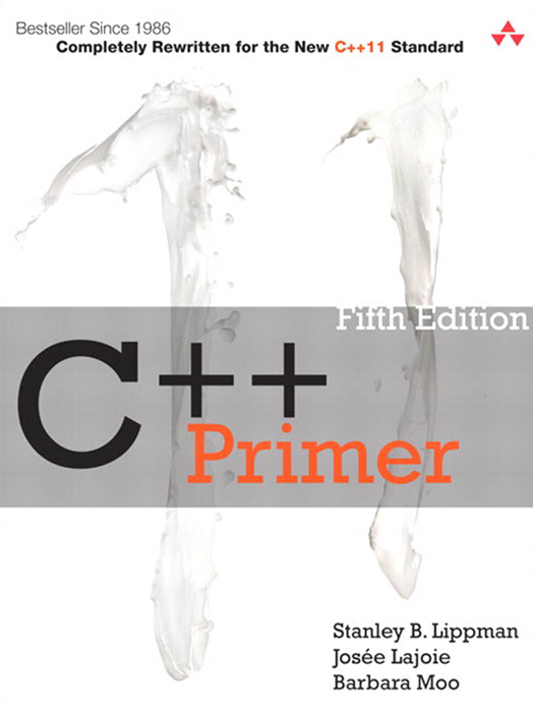
\includegraphics[width=0.8\textwidth]{day8_pm/img/1-cppprimer}
			\end{center}

		\end{column}
		\begin{column}{0.6\textwidth}
			\begin{itemize}
				\item \textbf{Title}: C++ Primer (Fifth Edition)
				\item \textbf{Authors}: Stanley B. Lippman, Josée Lajoie, and Barbara E. Moo
				\item \textbf{Publisher}: Addison-Wesley Professional
			\end{itemize}
		\end{column}
	\end{columns}
\end{frame}

\begin{frame}[fragile]{\emoji{books} Textbook}

	\begin{columns}
		\begin{column}{0.4\textwidth}
			\begin{center}
				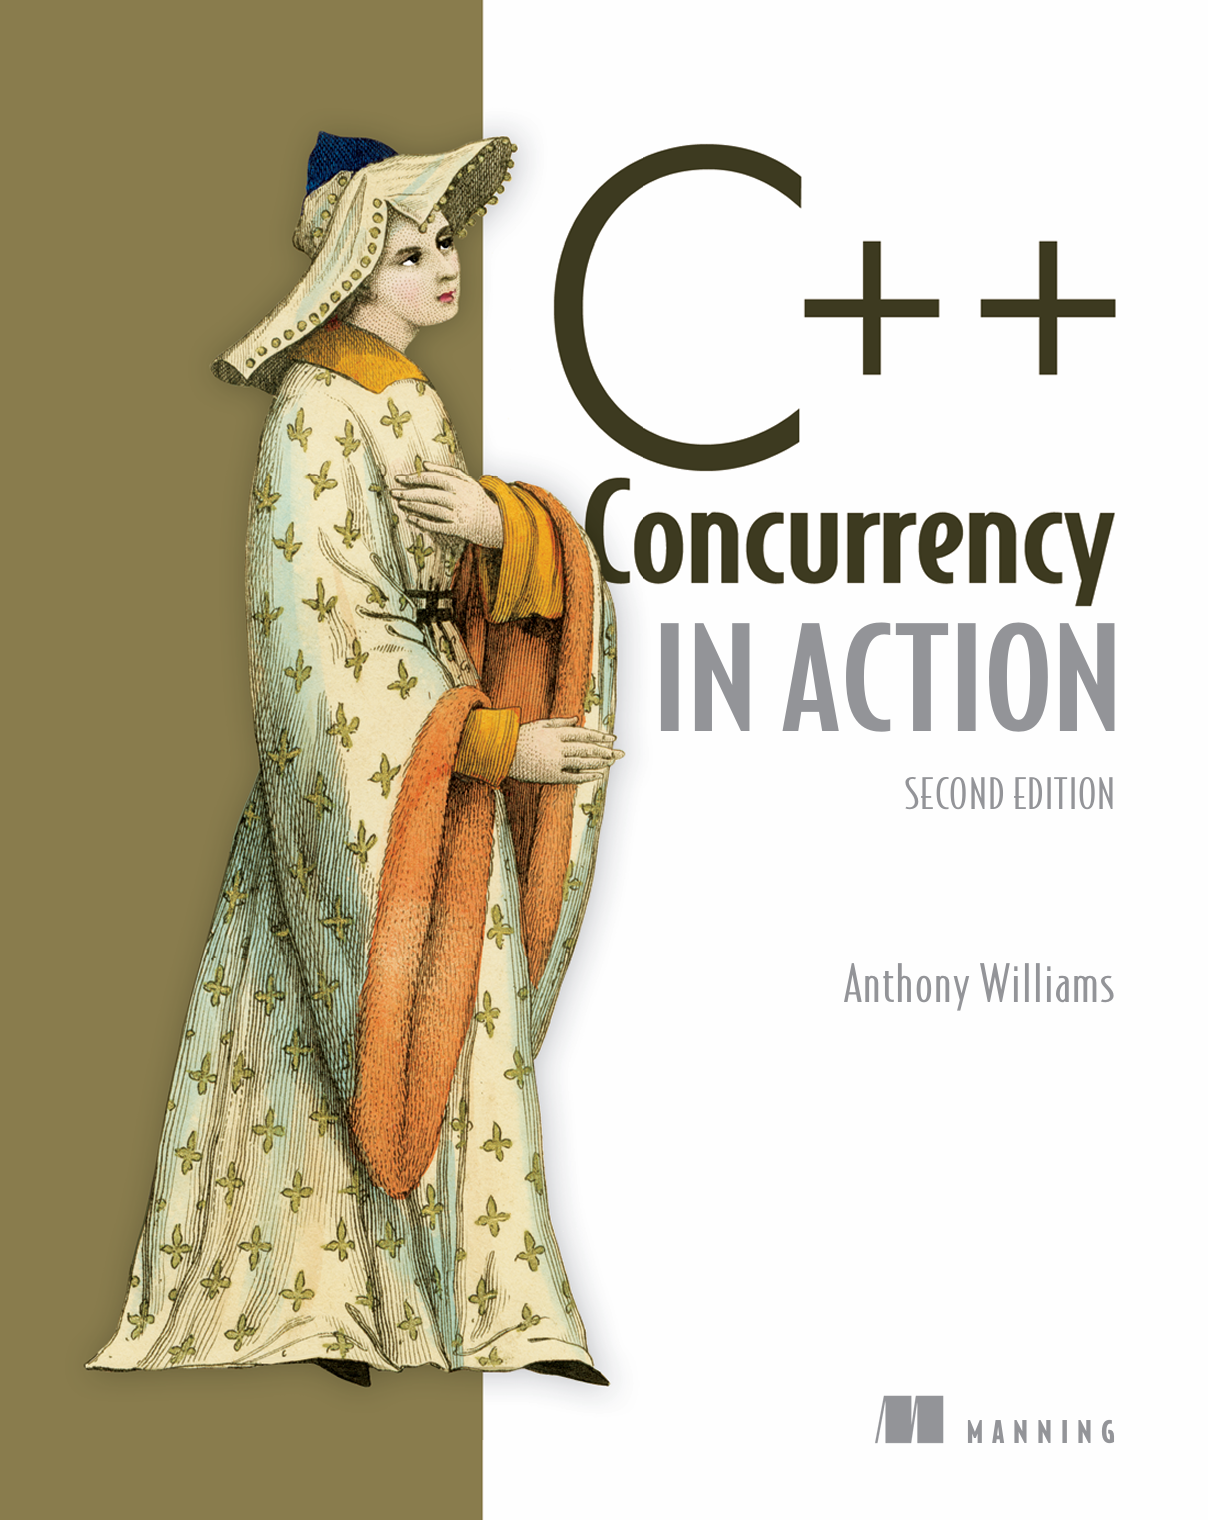
\includegraphics[width=0.8\textwidth]{day8_pm/img/1-ccia}
			\end{center}

		\end{column}
		\begin{column}{0.6\textwidth}
			\begin{itemize}
				\item \textbf{Title}: C++ Concurrency in Action (Second Edition)
				\item \textbf{Authors}: Anthony Williams
				\item \textbf{Publisher}: Manning Publications
			\end{itemize}
		\end{column}
	\end{columns}
\end{frame}

% Tips:遇到 C/C++ 语法问题,去 CPPREFERENCE 查找
\begin{frame}[fragile]{\emoji{light-bulb} Tips}
	\begin{itemize}
		\item \textbf{C/C++ Reference}: Use \textcolor{blue}{\href{https://en.cppreference.com/}{cppreference}} for syntax and library functions
		\item \textbf{Compiler Documentation}: Check your compiler's documentation for specific features and extensions (Example: \textcolor{blue}{\href{https://gcc.gnu.org/onlinedocs/gcc/Attributes.html}{GCC Attributes}})
		\item \textbf{Online Communities}: Engage with communities like Stack Overflow for troubleshooting and best practices
		\item \textbf{Source Codes}: You can copy from \verb|\river\hpc101\2025\day8\_pm| to your home directory for practice
	\end{itemize}
	\begin{minted}{bash}
cp -r /river/hpc101/2025/day8_pm ~/day8_pm
make
    \end{minted}
\end{frame}

% Tips:关于 HPC 学习:适应系统性学习的思维方式的同学,需要适应点状式学习的思维方式
\begin{frame}[fragile]{\emoji{light-bulb} Systematic vs. Problem-Driven Learning}
	\scriptsize
	\begin{columns}
		\begin{column}{0.45\textwidth}
			\textbf{Systematic Learning}
			\begin{itemize}
				\item Builds a structured knowledge network
				\item Driven by internal logic of disciplines
				\item Strong foundation, long-term benefits
				\item Limitation: Time-consuming, less adaptive
			\end{itemize}
		\end{column}
		\begin{column}{0.55\textwidth}
			\textbf{Problem-Driven Learning}
			\begin{itemize}
				\item Focuses on solving specific problems
				\item Knowledge acquisition is modular and need-based
				\item Quick results, highly focused
				\item Limitation: Fragmented knowledge, less depth
			\end{itemize}
		\end{column}
	\end{columns}
	\vspace{0.5cm}
	\textbf{Key Insight:} Effective learners adaptively combine both approaches, leveraging systematic learning for foundational understanding and problem-driven learning for practical application.

	% 知识像一张网或一棵树,你应当学会,能够从其上任何一个点出发

	\textbf{Knowledge is like a web or a tree, you should learn to start from any point on it.}

	%\normalsize
\end{frame}

% 本节课的内容大纲
\begin{frame}[fragile]{\emoji{book} Outline}
	\begin{enumerate}
		\item \textbf{C++ Quick Start}
		      \begin{itemize}
			      \item Object-oriented programming
			      \item Key differences between C++ and C
			      \item Containers and Algorithms
			      \item Lambda and Callable objects
			      \item Templates and Generic Programming
		      \end{itemize}
		\item \textbf{C++ Concurrency Overview}: \texttt{<thread>}, \texttt{<mutex>}, \texttt{<condition\_variable>}, \texttt{<execution>}
		\item \textbf{Summary and Framework Selection}
	\end{enumerate}
\end{frame}

% 预修要求:C 语言,否则请先跳过本节课,补习 C 语言基础
\begin{frame}[fragile]{\emoji{warning} Prerequisites}
	\begin{itemize}
		\item \textbf{C Language Proficiency}: Basic understanding of C syntax and concepts
		\item \textbf{Familiarity with Pointers}: Understanding of pointers, memory management, and basic data structures
		\item \textbf{Basic Programming Constructs}: Loops, conditionals, functions, and arrays
	\end{itemize}
\end{frame}

\section{C++ Quick Start}

\subsection{Object-Oriented Programming}

% 简单对比过程式编程和面向对象编程
\begin{frame}[fragile]{Procedural vs Object-Oriented Programming}
	\begin{columns}
		\begin{column}{0.5\textwidth}
			\textbf{C: Procedural Programming}
			\begin{itemize}
				\item Focus on functions and data
				\item Functions operate on data structures
				\item No built-in support for encapsulation or inheritance
			\end{itemize}
		\end{column}
		\begin{column}{0.5\textwidth}
			\textbf{C++: Object-Oriented Programming}
			\begin{itemize}
				\item Combines data and functions into classes
				\item Supports encapsulation, inheritance, and polymorphism
				\item Provides a more modular and reusable code structure
			\end{itemize}
		\end{column}
	\end{columns}

	A class defines a type \textbf{along with a collection of operations that are related to that type}.
\end{frame}

\begin{frame}[fragile]{Procedural vs Object-Oriented Programming}
	\begin{columns}
		\begin{column}{0.5\textwidth}
			\textbf{C Struct (Data \textcolor{orange}{and} Functions)}
			\begin{minted}{c}
struct Student {
    char name[50];
    int age;
    float gpa;
};
void print_student(struct Student s) {
    printf("Name: %s\n", s.name);
    printf("Age: %d\n", s.age);
    printf("GPA: %.2f\n", s.gpa);
}
int main() {
    struct Student alice = {"Alice", 20, 3.8};
    print_student(alice);
    return 0;
}
			\end{minted}
		\end{column}
		\begin{column}{0.5\textwidth}
			\textbf{C++ Class (Data \textcolor{orange}{with} Functions)}
			\begin{minted}{cpp}
class Student {
private:
    string name;
    int age;
    float gpa;
public:
    Student(string n, int a, float g)
        : name(n), age(a), gpa(g) {}
    void print() {
        cout << "Name: " << name << endl;
        cout << "Age: " << age << endl;
        cout << "GPA: " << gpa << endl;
    }
};
int main() {
    Student alice("Alice", 20, 3.8);
    alice.print();  // Object calls its own method
    return 0;
}
			\end{minted}
		\end{column}
	\end{columns}
\end{frame}

\begin{frame}[fragile]{Abstract Data Types}
	The fundamental ideas behind classes are \textbf{data abstraction} and \textbf{encapsulation}.

	\begin{itemize}
		\item \textbf{Data Abstraction}: Separation of \textcolor{blue}{interface} and \textcolor{orange}{implementation}
		\item \textbf{Encapsulation}: Enforces this separation by hiding implementation details
		\item Together, they define an \textbf{Abstract Data Type (ADT)}
	\end{itemize}

	\vspace{0.3em}
	\begin{columns}
		\begin{column}{0.5\textwidth}
			\textbf{Interface (What users see)}
			\begin{itemize}
				\item Public operations users can execute
				\item Contract of what the class does
				\item Think abstractly about behavior
			\end{itemize}
		\end{column}
		\begin{column}{0.5\textwidth}
			\textbf{Implementation (Hidden details)}
			\begin{itemize}
				\item Data members
				\item Function bodies
				\item Internal helper functions
			\end{itemize}
		\end{column}
	\end{columns}
\end{frame}

\begin{frame}[fragile]{Abstract Data Type: An Example}
	\begin{columns}
		\begin{column}{0.5\textwidth}
			\textbf{Interface (Public)}
			\begin{itemize}
				\item \texttt{Book(title, author, pages, count)} - Constructor
				\item \texttt{isAvailable()} - Check availability
				\item \texttt{addCopies(num)} - Add copies
			\end{itemize}
			\vspace{0.3em}
			\textbf{Users care about:} \\
			\textit{What} operations are available, not \textit{how} they work
		\end{column}
		\begin{column}{0.5\textwidth}
			\begin{minted}{cpp}
class Book {
private:  // Implementation (Hidden)
    string title;
    string author;
    int pages;
    int count;
public:   // Interface (Visible)
    Book(string t, string a, int p, int c);
    bool isAvailable() const;
    void addCopies(int num);
};
            \end{minted}
		\end{column}
	\end{columns}
\end{frame}

\begin{frame}[fragile]{Abstract Data Types: Key Benefits}

	\begin{columns}
		\begin{column}{0.5\textwidth}
			\textbf{For Class Designers:}
			\begin{itemize}
				\item Focus on \textbf{how} the class is implemented
				\item Can change implementation without breaking user code
				\item Control access to internal data
			\end{itemize}
		\end{column}
		\begin{column}{0.5\textwidth}
			\textbf{For Class Users:}
			\begin{itemize}
				\item Don't need to know \textbf{how} the type works
				\item Think abstractly about \textbf{what} the type does
				\item Use the interface without worrying about details
			\end{itemize}
		\end{column}
	\end{columns}
\end{frame}

\begin{frame}[fragile]{Class: Definition}
	\begin{minted}[fontsize=\scriptsize]{cpp}
class ClassName {
public:  // Public interface
    ClassName();  // Constructor
    ~ClassName(); // Destructor
    void publicMethod();  // Public method
private: // Private implementation details
    int privateData;  // Private data member
    void privateMethod();  // Private method
protected: // Protected members (accessible by derived classes)
    int protectedData;  // Protected data member
};
    \end{minted}
\end{frame}

% 介绍类的实例化
\begin{frame}[fragile]{Class: Instantiation}
	Instantiate a class to create an object
	\begin{itemize}
		\item Use the class name as a type
		\item Call the constructor to initialize the object
		\item Objects are instances of the class
	\end{itemize}
	\begin{minted}{cpp}
int main() {
    Point p(10, 20);  // Create an object of Point
    p.display();      // Call public method
    return 0;
}
    \end{minted}
\end{frame}

\begin{frame}[fragile]{Class: \texttt{this} pointer}
	A special pointer that refers to the current object

	\begin{itemize}
		\item Used inside class methods to access members of the current object
		\item Helps distinguish between member variables and parameters with the same name
	\end{itemize}

	\begin{minted}{cpp}
class Point {
private:
    int x, y;
public:
    Point(int x, int y) {
        this->x = x;  // Use this to refer to member variable
        this->y = y;  // Use this to refer to member variable
    }
};
    \end{minted}
\end{frame}

% 介绍右值引用
\begin{frame}[fragile]{Class: Rvalue References}
	\textbf{Rvalue Reference:} A new reference type introduced in C++11
	\begin{itemize}
		\item Allows binding to temporary objects (rvalues)
		\item Syntax: \texttt{Type\&\&} (double ampersand)
		\item Enables move semantics and perfect forwarding
	\end{itemize}

	\begin{minted}{cpp}
A& a_lref = a; // lvalue reference
A&& a_rref = a; // rvalue reference
	\end{minted}

	See: \textcolor{blue}{\href{https://www.open-std.org/jtc1/sc22/wg21/docs/papers/2006/n2027.html}{A Brief Introduction to Rvalue References - Bjarne Stroustrup}}
\end{frame}

% 介绍移动语义
\begin{frame}[fragile]{Class: Move Semantics}
	\begin{minted}{cpp}
template <class T> swap(T& a, T& b)
{
    T tmp(a);   // now we have two copies of a
    a = b;      // now we have two copies of b
    b = tmp;    // now we have two copies of tmp (aka a)
}

template <class T> swap(T& a, T& b) {
    T tmp = std::move(a);
    a = std::move(b);
    b = std::move(tmp);
}
    \end{minted}
\end{frame}

% 介绍 move()
\begin{frame}[fragile]{Class: \texttt{std::move}}
	\textbf{std::move:} A utility function that casts an object to an rvalue reference
	\begin{itemize}
		\item Indicates that the object can be moved
		\item Does not actually move anything, just changes the type
	\end{itemize}

	\textbf{Prototype:}
	\begin{minted}{cpp}
template <class T>
typename remove_reference<T>::type&&
move(T&& a)
{
    return a;
}
    \end{minted}
	It is now up to client code to overload key functions on whether their argument is an lvalue or rvalue.
\end{frame}

% 介绍拷贝
\begin{frame}[fragile]{Class: Copying Objects}
	C++ allows copying objects using the copy constructor
	\begin{itemize}
		\item Copy constructor: when an object is passed by value or returned from a function
		\item Default copy constructor performs a shallow copy (member-wise copy)
		\item Custom copy constructor can be defined for deep copying
	\end{itemize}

	\begin{columns}
		\begin{column}{0.5\textwidth}
			\begin{minted}{cpp}
class Point {
public:
    // Custom copy constructor
    Point(const Point& other) {
        x = other.x;
        y = other.y;
    }
};
\end{minted}
		\end{column}
		\begin{column}{0.5\textwidth}
			\begin{minted}{cpp}
Point p1(10, 20);
Point p2 = p1;  // Calls copy constructor
p2.display();   // Displays copied point
    \end{minted}
		\end{column}
	\end{columns}
\end{frame}

% 介绍移动
\begin{frame}[fragile]{Class: Moving Objects}
	C++11 introduced move semantics to optimize resource management
	\begin{itemize}
		\item Move constructor transfers ownership of resources from one object to another
		\item Avoids deep copying, improving performance for temporary objects
		\item Use \texttt{std::move} to indicate an object can be moved
	\end{itemize}

	\begin{columns}
		\begin{column}{0.5\textwidth}
			\begin{minted}{cpp}
class Point {
public:
    // Move constructor
    Point(Point&& other) noexcept {
        x = other.x;
        y = other.y;
        other.x = 0;  // Leave moved-from object in a valid state
        other.y = 0;
    }
};
\end{minted}
		\end{column}
		\begin{column}{0.5\textwidth}
			\begin{minted}{cpp}
Point p1(10, 20);
Point p2 = std::move(p1);  // Calls move constructor
p2.display();               // Displays moved point
            \end{minted}
		\end{column}
	\end{columns}
\end{frame}


% 介绍析构
\begin{frame}[fragile]{Class: Destructor}
	\textbf{Destructor:} A special member function called when an object goes out of scope or is deleted
	\begin{itemize}
		\item Cleans up resources (memory, file handles, etc.)
		\item Automatically called when the object is destroyed
		\item Can be defined to perform custom cleanup actions
	\end{itemize}

	\begin{columns}
		\begin{column}{0.5\textwidth}
			\begin{minted}{cpp}
class Point {
public:
    // Destructor
    ~Point() {
        cout << "Point(" << x << ", " << y << ") destroyed" << endl;
    }
};
        \end{minted}
		\end{column}
		\begin{column}{0.5\textwidth}
			\begin{minted}{cpp}
int main() {
    Point p(10, 20);  // Constructor called
    p.display();      // Displays point
    return 0;        // Destructor called automatically
}
    \end{minted}
		\end{column}
	\end{columns}
\end{frame}



\begin{frame}[fragile]{Encapsulation}
	\textbf{Encapsulation enforces the separation of interface and implementation}
	\begin{itemize}
		\item \textbf{Hide Implementation}: Users cannot access internal details
		\item \textbf{Control Access}: Define exactly how others can use your class
		\item \textbf{Maintainability}: Change implementation without breaking user code
		\item \textbf{Data Protection}: Prevent accidental or malicious modification
	\end{itemize}

\end{frame}

\begin{frame}[fragile]{Encapsulation: Access specifiers}
	\begin{minted}[fontsize=\scriptsize]{cpp}
class BankAccount {
private:    // Only this class can access
    double balance;
public:     // Anyone can access
    void deposit(double amount) {
        if (amount > 0) balance += amount;  // Safe deposit
    }
    double getBalance() const { return balance; }  // Read-only access
protected:  // This class and its children can access
    void setBalance(double newBalance) { balance = newBalance; }
};
    \end{minted}
	\begin{itemize}
		\item \texttt{struct}: Members are \textbf{public} by default - less encapsulation
		\item \texttt{class}: Members are \textbf{private} by default - enforces encapsulation
	\end{itemize}
\end{frame}

\begin{frame}[fragile]{Inheritance: Building on Existing Code}
	\textbf{Like a Family Tree:} Children inherit traits from parents

	\begin{columns}
		\begin{column}{0.3\textwidth}
			\textbf{Base Class (Parent)}
			\begin{minted}{cpp}
class Animal {
protected:
    string name;
public:
    Animal(string n) : name(n) {}
    void eat() { cout << name << " is eating\n"; }
    virtual void makeSound() { cout << name << " makes a sound\n"; }
};
    \end{minted}
		\end{column}
		\begin{column}{0.7\textwidth}
			\textbf{Derived Class (Child)}
			\begin{minted}{cpp}
class Dog : public Animal {
public:
    Dog(string n) : Animal(n) {}  // Call parent constructor
    void makeSound() override {        // Override parent method
        cout << name << " barks: Woof!\n";
    }
    void wagTail() { cout << name << " wags tail\n"; }  // New method
};

int main() {
    Dog buddy("Buddy");
    buddy.eat();        // Inherited from Animal
    buddy.makeSound();  // Dog's own version
    buddy.wagTail();    // Dog-specific behavior
    return 0;
}
    \end{minted}
		\end{column}
	\end{columns}
\end{frame}

\begin{frame}[fragile]{Polymorphism: One Interface, Many Forms}
	\textbf{Like a Universal Remote:} Same buttons, different devices

	\begin{columns}
		\begin{column}{0.6\textwidth}
			\begin{minted}{cpp}
class Shape {
public:
    virtual double area() = 0;  // Pure virtual function
    virtual ~Shape() = default;
};
class Circle : public Shape {
    double radius;
public:
    Circle(double r) : radius(r) {}
    double area() override { return 3.14159 * radius * radius; }
};
class Rectangle : public Shape {
    double width, height;
public:
    Rectangle(double w, double h) : width(w), height(h) {}
    double area() override { return width * height; }
};
    \end{minted}
		\end{column}
		\begin{column}{0.4\textwidth}

			\begin{minted}{cpp}
vector<unique_ptr<Shape>> shapes;
shapes.push_back(make_unique<Circle>(5.0));
shapes.push_back(
    make_unique<Rectangle>(4.0, 6.0));
for (auto& shape : shapes) {
    cout << "Area: " << shape->area()
         << endl;
    // Calls correct method
}
    \end{minted}
		\end{column}
	\end{columns}
\end{frame}

\subsection{The Basics}

\begin{frame}[fragile]{I/O Streams: Compared to C Standard I/O}
	\begin{columns}
		\begin{column}{0.5\textwidth}
			\textbf{C Style}
			\begin{minted}{c}
#include <stdio.h>
#include <stdlib.h>

void print_msg(void) {
    printf("Hello from C!\n");
}

int main() {
    FILE* fp = fopen("test.txt", "r");
    if (fp) {
        // Manual resource management
        char line[100];
        while (fgets(line, 100, fp) != NULL) {
            printf("%s", line);
        }
        fclose(fp);
    }
    return 0;
}
			\end{minted}
		\end{column}
		\begin{column}{0.5\textwidth}
			\textbf{C++ Style}
			\begin{minted}{cpp}
#include <iostream>
#include <fstream>

void print_msg() {
    std::cout << "Hello from C++!" << std::endl;
}

int main() {
    std::ifstream file("test.txt");
    if (file.is_open()) {
        // Automatic resource management
        std::string line;
        while (std::getline(file, line)) {
            std::cout << line << std::endl;
        }
    }
    return 0;
}
			\end{minted}
		\end{column}
	\end{columns}
\end{frame}

% 介绍 C++ 的引用和指针
\begin{frame}[fragile]{References}
	\begin{columns}
		\begin{column}{0.5\textwidth}
			\textbf{C Pointers}
			\begin{minted}{c}
void swap_c(int* a, int* b) {
    int temp = *a;
    *a = *b;
    *b = temp;
}
int main() {
    int x = 5, y = 10;
    swap_c(&x, &y);  // Pass addresses
    printf("x=%d, y=%d\n", x, y);
    return 0;
}
			\end{minted}
		\end{column}
		\begin{column}{0.5\textwidth}
			\textbf{C++ References}
			\begin{minted}{cpp}
void swap_cpp(int& a, int& b) {
    int temp = a;
    a = b;
    b = temp;
}
int main() {
    int x = 5, y = 10;
    swap_cpp(x, y);  // Direct pass
    cout << "x=" << x << ", y=" << y << endl;
    return 0;
}
			\end{minted}
		\end{column}
	\end{columns}

	\vspace{0.5em}
	\begin{itemize}
		\item References are \textbf{aliases} for existing objects: \texttt{int a; int\& b = a;}
		\item References must be initialized and cannot be reassigned
	\end{itemize}
\end{frame}

% 本页展示 C++ 的所有运算符
\begin{frame}[fragile]{C++ Operators and Keywords (From \textcolor{blue}{\href{https://en.cppreference.com/w/cpp/language/}{cppreference.com}})}
	\begin{columns}
		\begin{column}{0.6\textwidth}
			\begin{figure}
				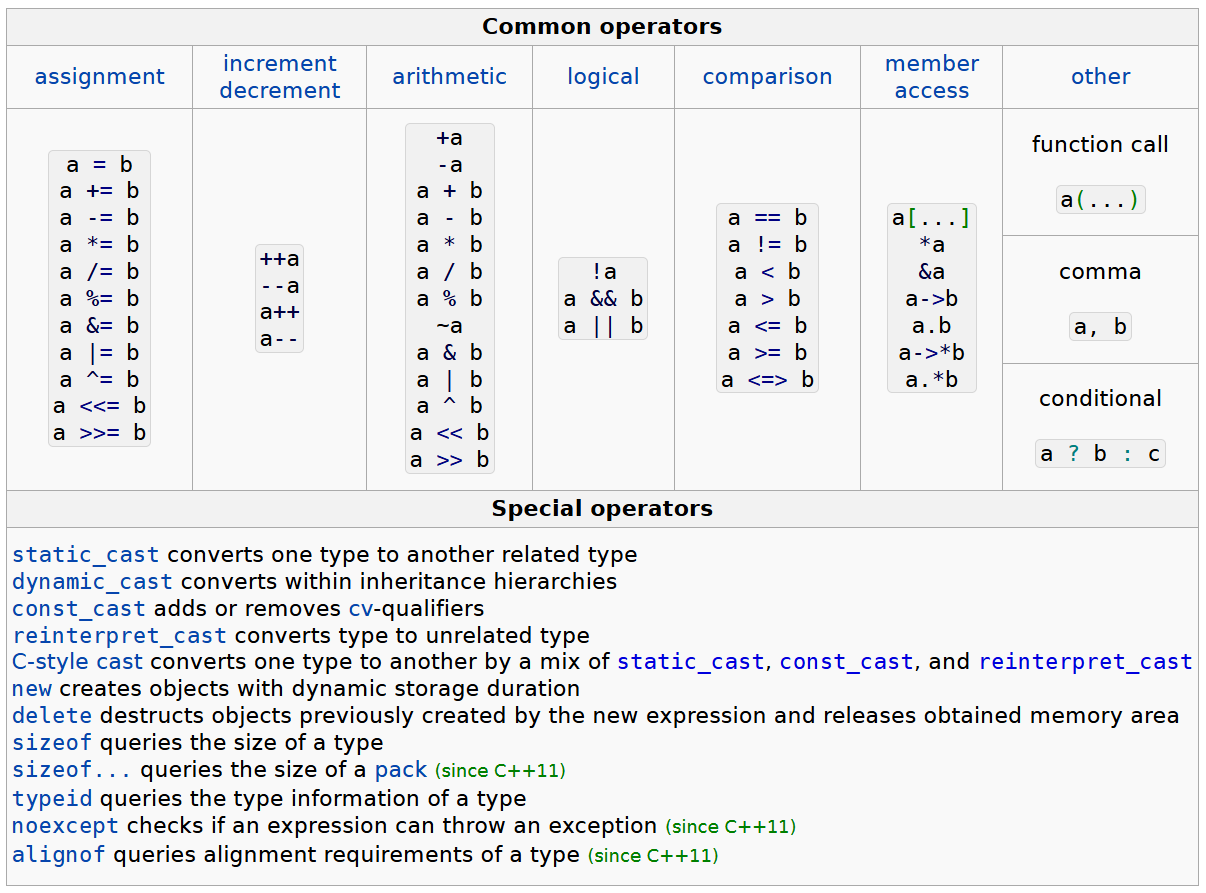
\includegraphics[width=\textwidth]{day8_pm/img/1-operators}
			\end{figure}
		\end{column}
		\begin{column}{0.4\textwidth}
			\begin{figure}
				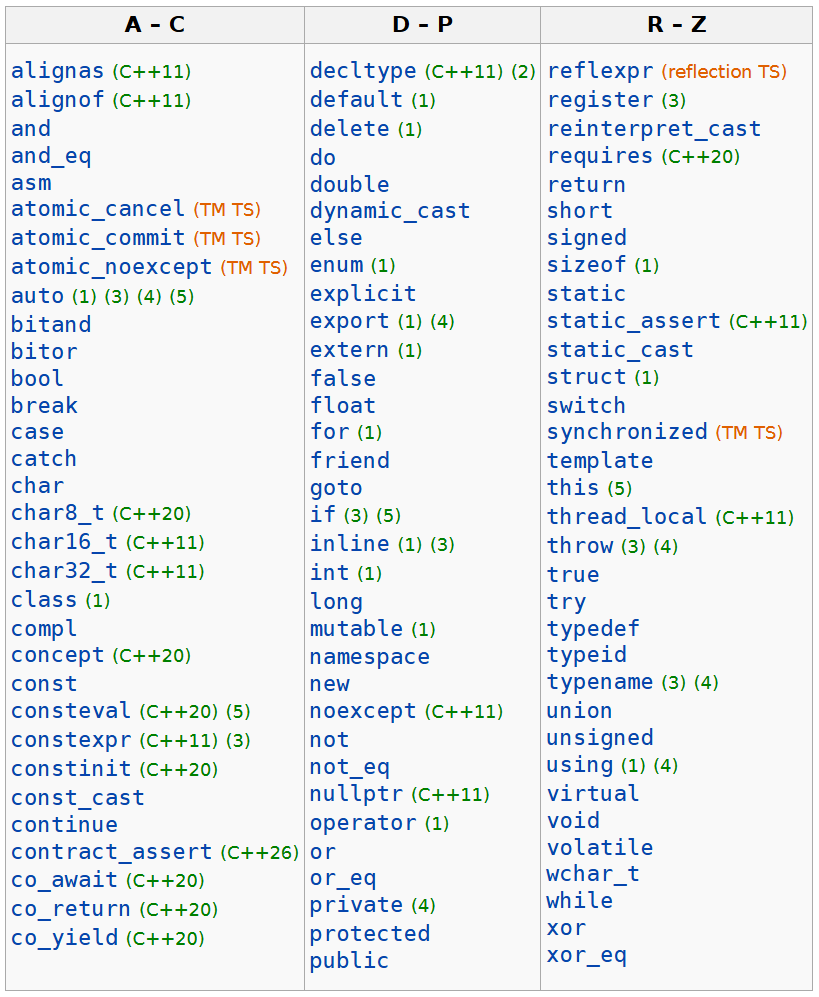
\includegraphics[width=0.9\textwidth]{day8_pm/img/1-keywords}
			\end{figure}
		\end{column}
	\end{columns}
\end{frame}

\begin{frame}[fragile]{C++ Operators and Keywords}
	We'll meet some new friends in this class:
	\begin{itemize}
		\item \textbf{I/O}:  \texttt{>>}, \texttt{<<}
		\item \textbf{Memory}: \texttt{new}, \texttt{delete}, \texttt{new[]}, \texttt{delete[]}
		\item \textbf{Type System}: \texttt{auto}, \texttt{decltype}, \texttt{using}, \texttt{operator}
		\item \textbf{Class}: \texttt{::}, \texttt{public}, \texttt{private}, \texttt{protected}, \texttt{friend}, \texttt{virtual}, \texttt{override}, \texttt{final}
	\end{itemize}
\end{frame}

% 上页给出代码对比,本页给出讲解
\begin{frame}[fragile]{I/O Streams}
	\begin{table}[]
		% table of streams: i, o, io; file, string, c
		\begin{tabular}{cccc}
			\hline
			\textbf{Type} & \textbf{Input}         & \textbf{Output}                             & \textbf{Both}         \\ \hline
			standard      & \texttt{cin}           & \texttt{cout}, \texttt{cerr}, \texttt{clog} &                       \\ \hline
			File          & \texttt{ifstream}      & \texttt{ofstream}                           & \texttt{fstream}      \\ \hline
			String        & \texttt{istringstream} & \texttt{ostringstream}                      & \texttt{stringstream} \\ \hline
		\end{tabular}
	\end{table}

	\textbf{Benefits of C++ Streams:}
	\begin{itemize}
		\item Type safety and flexibility
		\item Easier to read and maintain code
		\item Automatic resource cleanup when objects go out of scope
	\end{itemize}
\end{frame}

% 给出一个 sstream 的例子,以展示相比 C 的优势
\begin{frame}[fragile]{I/O Streams: Example}
	\textbf{String Streams:} Like a string that can be read/written like a file
	\begin{minted}{cpp}
#include <sstream>
#include <iostream>

void example_string_stream() {
    std::stringstream ss;
    ss << "The answer is " << 42;
    std::string result = ss.str();
    std::cout << result << std::endl;
}
    \end{minted}

	\textbf{Benefits:}
	\begin{itemize}
		\item Concise syntax for formatting strings
		\item No need for manual memory management
		\item Can be used with any type that supports stream operators
	\end{itemize}
\end{frame}

% 介绍命名空间,标准库的所有名字都在命名空间 std 中
\begin{frame}[fragile]{Namespaces}
	\begin{itemize}
		\item C++ uses namespaces to avoid \textbf{name collisions}
		\item \textbf{Standard library} functions and classes are in the \texttt{std} namespace
		\item Use \texttt{using namespace std;} to avoid prefixing with \texttt{std::} (should be avoided in header files and large projects)
	\end{itemize}
	\textbf{Example:}
	\begin{minted}[fontsize=\scriptsize]{cpp}
#include <iostream>
using namespace std;
cout << "Hello, World!" << endl;
        \end{minted}
\end{frame}

% 介绍运算符语法
\begin{frame}[fragile]{Class: Operator overloading}
	\begin{itemize}
		\item C++ lets us define what the operators mean \textbf{when applied to objects of class type}.
		\item They are \textbf{special functions} with concise syntax
		\item Can be \textbf{overloaded} to provide custom behavior for user-defined types
		\item In a user-defined operator overload, \textbf{any type} can be used as return type (including \texttt{void})
		\item Operators for \textbf{primitive types} like \texttt{int}, \texttt{float}, etc. cannot be overloaded
	\end{itemize}

	\textbf{Syntax:}
	\begin{minted}[fontsize=\scriptsize]{cpp}
<return_type> operator<operator_symbol>(<parameters>) { /* Implementation */ }
// An illustration of overloading the + operator
int operator+(int a, int b) { return a + b; }
    \end{minted}
\end{frame}

% 以 I/O 操作符为例,介绍运算符重载:巧妙地通过重载,利用了移位运算符的语法
\begin{frame}[fragile]{Class: Operator overloading}
	\textbf{Why Overload I/O Operators?}
	\begin{itemize}
		\item Makes it easy to print custom objects
		\item Uses existing syntax (\texttt{<<} and \texttt{>>}) for a natural feel
	\end{itemize}

	\textbf{Prototype}
	% A prototype demonstrating how stream class overloads the I/O operators
	\begin{minted}{cpp}
template< class Traits >
basic_ostream<char, Traits>&
    operator<<( basic_ostream<char, Traits>& os, const char* s );
basic_istream& operator>>( int& value );
    \end{minted}
	\textbf{Example Usage}:
	\begin{minted}{cpp}
cout << "Hello, World!" << endl;
cin >> user_input;
    \end{minted}
\end{frame}

\begin{frame}[fragile]{Function Overloading: Same Name, Different Parameters}
	\textbf{Function Overloading:} Multiple functions with the same name but different parameters

	\begin{itemize}
		\item C++ allows multiple functions with the same name
		\item Functions must differ in number or type of parameters
		\item Compiler chooses the best match based on arguments
		\item Return type alone is \textbf{not} enough to distinguish functions
	\end{itemize}
\end{frame}

\begin{frame}[fragile]{Function Overloading vs C Naming Conventions}
	\begin{columns}
		\begin{column}{0.5\textwidth}
			\textbf{C Style: Different Names}
			\begin{minted}[fontsize=\tiny]{c}
#include <stdio.h>
#include <math.h>

// Need different names for each type
int abs_int(int x) { return x < 0 ? -x : x; }
double abs_double(double x) { return x < 0.0 ? -x : x; }
float abs_float(float x) { return x < 0.0f ? -x : x; }
int main() {
    printf("%d\n", abs_int(-5));
    printf("%.2f\n", abs_double(-3.14));
    printf("%.2f\n", abs_float(-2.5f));
    return 0;
}
            \end{minted}
		\end{column}
		\begin{column}{0.5\textwidth}
			\textbf{C++ Style: Overloaded Functions}
			\begin{minted}[fontsize=\tiny]{cpp}
#include <iostream>
#include <cmath>
using namespace std;
// Same name, different parameters
int abs(int x) { return x < 0 ? -x : x; }
double abs(double x) { return x < 0.0 ? -x : x; }
float abs(float x) { return x < 0.0f ? -x : x; }

int main() {
    cout << abs(-5) << endl;   // Calls abs(int)
    cout << abs(-3.14) << endl;// Calls abs(doubl)
    cout << abs(-2.5f) << endl;// Calls abs(float)
    return 0;
}
            \end{minted}
		\end{column}
	\end{columns}
\end{frame}

\begin{frame}[fragile]{Function Overloading: Rules and Best Practices}
	\textbf{Overloading Rules:}
	\begin{itemize}
		\item Functions must differ in \textbf{number} or \textbf{type} of parameters
		\item \textbf{const} and non-const parameters are considered different
		\item Reference and non-reference parameters are different
		\item Return type alone cannot distinguish overloaded functions
	\end{itemize}

	\textbf{Example of Valid Overloads:}
	\begin{minted}[fontsize=\scriptsize]{cpp}
void func(int x);                    // Version 1
void func(double x);                 // Version 2: different type
void func(int x, int y);             // Version 3: different number of para
void func(const int& x);             // Version 4: different parameter form
// void func(int x) { return 5; }    // ERROR: Only return type differs
    \end{minted}

	\textbf{Best Practice:} Use overloading for functions that perform \textbf{similar operations} on different types
\end{frame}

\subsection{Containers and Algorithms}
\begin{frame}[fragile]{STL: Your Programming Toolbox}
	\textbf{Standard Template Library (STL):}
	\begin{itemize}
		\item \textbf{Containers}: Ready-made data structures (like toolboxes)
		\item \textbf{Algorithms}: Common operations (like tools)
		\item \textbf{Iterators}: Ways to access container elements (like handles)
	\end{itemize}

	\vspace{0.5em}
	\textbf{Why use STL instead of arrays?}
	\begin{itemize}
		\item \textbf{Safety}: Automatic bounds checking and memory management
		\item \textbf{Convenience}: Built-in functions for common operations
		\item \textbf{Performance}: Optimized implementations
		\item \textbf{Compatibility}: Works seamlessly with C++ features
	\end{itemize}
\end{frame}

\begin{frame}[fragile]{Common Containers: Your Data Storage Options}
	\begin{columns}
		\begin{column}{0.5\textwidth}
			\textbf{Vector: Dynamic Array}
			\begin{minted}{cpp}
vector<int> numbers;
// Add elements
numbers.push_back(10);
numbers.push_back(20);
numbers.push_back(30);
// Access elements
cout << "First: " << numbers[0] << endl;
cout << "Size: " << numbers.size() << endl;
// Iterate through all
for (int num : numbers) { cout << num << " "; }
			\end{minted}
		\end{column}
		\begin{column}{0.5\textwidth}
			\textbf{Map: Key-Value Storage}
			\begin{minted}{cpp}
map<string, int> scores;
// Add key-value pairs
scores["Alice"] = 95;
scores["Bob"] = 87;
scores["Charlie"] = 92;
// Look up values
cout << "Alice's score: "
            << scores["Alice"] << endl;
// Check if key exists
if (scores.find("David") != scores.end()) {
    cout << "David found\n";
} else {
    cout << "David not found\n";
}
			\end{minted}
		\end{column}
	\end{columns}
\end{frame}

\begin{frame}[fragile]{Algorithms: Ready-Made Solutions}
	\textbf{Common algorithms you'll use:}
	\begin{table}[]
		\begin{tabular}{|l|l|}
			\hline
			\textbf{Category}       & \textbf{Algorithms}                                                                  \\ \hline
			\textbf{Sorting}        & \texttt{sort}, \texttt{stable\_sort}, \texttt{partial\_sort}, \texttt{nth\_element}  \\ \hline
			\textbf{Searching}      & \texttt{find}, \texttt{binary\_search}, \texttt{lower\_bound}, \texttt{upper\_bound} \\ \hline
			\textbf{Modifying}      & \texttt{copy}, \texttt{swap}, \texttt{replace}, \texttt{fill}, \texttt{transform}    \\ \hline
			\textbf{Set Operations} & \texttt{set\_union}, \texttt{set\_intersection}, \texttt{set\_difference}            \\ \hline
			\textbf{Numeric}        & \texttt{accumulate}, \texttt{inner\_product}, \texttt{adjacent\_difference}          \\ \hline
		\end{tabular}
	\end{table}
\end{frame}

\begin{frame}[fragile]{Algorithms: Ready-Made Solutions}
	\begin{minted}[fontsize=\scriptsize]{cpp}
vector<int> numbers = {64, 34, 25, 12, 22, 11, 90};
// Sort the vector
sort(numbers.begin(), numbers.end());
cout << "Sorted: ";
for (int n : numbers) cout << n << " ";
cout << endl;
// Find an element
auto it = find(numbers.begin(), numbers.end(), 25);
if (it != numbers.end()) {
    cout << "Found 25 at position: "
                << (it - numbers.begin()) << endl;
}
// Count elements greater than 30
int count = count_if(numbers.begin(), numbers.end(),
    [](int n) { return n > 30; });
cout << "Numbers > 30: " << count << endl;
    \end{minted}
\end{frame}

\begin{frame}[fragile]{More on STL Algorithms}
	\begin{figure}
		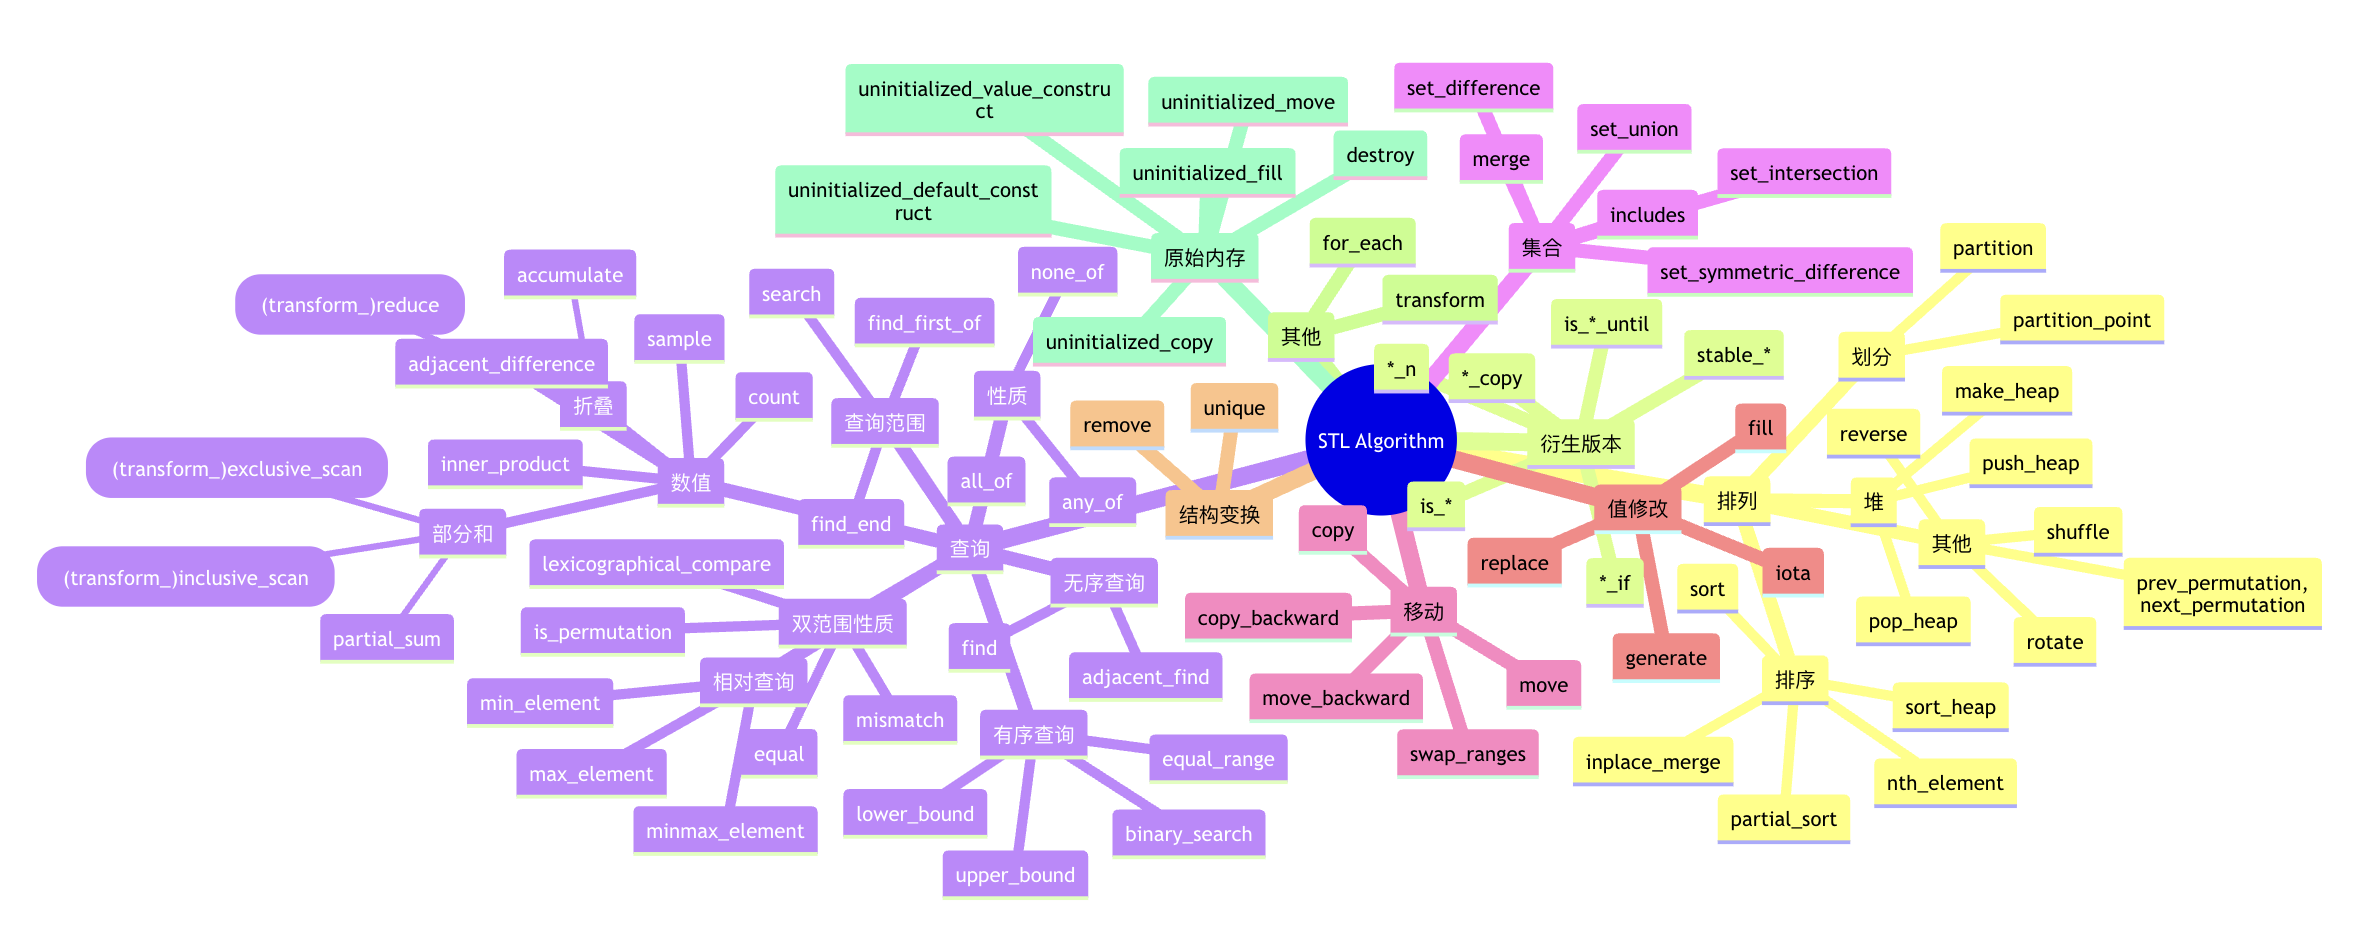
\includegraphics[width=\textwidth]{day8_pm/img/2-algorithms}
	\end{figure}
\end{frame}

\begin{frame}[fragile]{More on STL Algorithms}
	\textcolor{blue}{\href{https://www.youtube.com/watch?v=2olsGf6JIkU&ab_channel=CppCon}{CppCon 2018: 105 STL Algorithms in Less Than an Hour}}
	\begin{figure}
		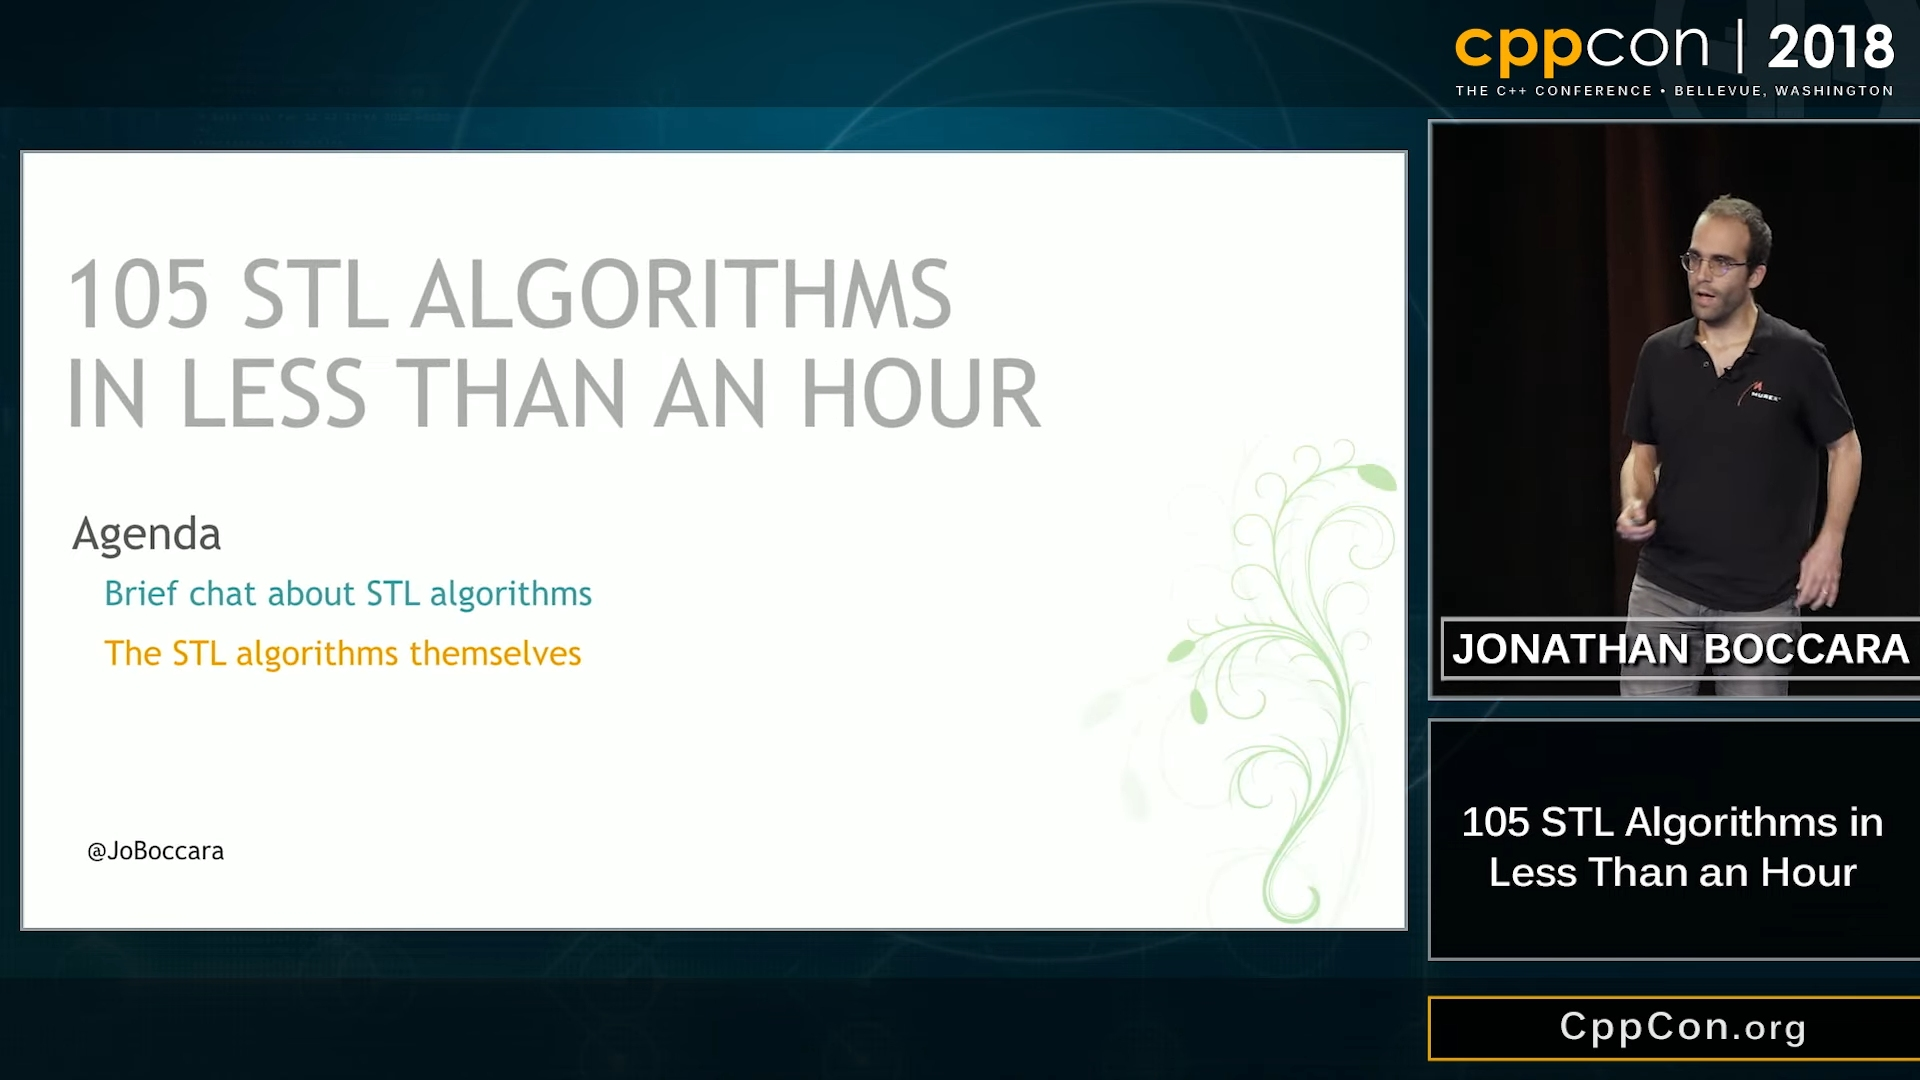
\includegraphics[width=0.7\textwidth]{day8_pm/img/2-cppcon2018}
	\end{figure}
\end{frame}

\begin{frame}[fragile]{Containers vs C Arrays: The Upgrade}
	\begin{columns}
		\begin{column}{0.5\textwidth}
			\textbf{C Arrays (Manual Everything)}
			\begin{minted}{c}
int arr[] = {1, 3, 2};
int size = 0;
// must write your compare function
qsort(ints, size, sizeof(int), compare_ints);
for (int i = 0; i < size; i++) {
    printf("%d ", arr[i]);
}
			\end{minted}
		\end{column}
		\begin{column}{0.5\textwidth}
			\textbf{C++ Containers (Automatic)}
			\begin{minted}{cpp}
// Dynamic size, automatic memory
vector<int> arr = {1, 3, 2};
sort(arr.begin(), arr.end());
for (int num : arr) {
    cout << num << " ";
}
			\end{minted}
		\end{column}
	\end{columns}

	\vspace{0.5em}
	\textbf{Benefits:} Safer, shorter, and often faster code!
\end{frame}

\subsection{Essential Features for Concurrency}
\begin{frame}[fragile]{Callable Objects}
	\textbf{Function Call Operator}
	\begin{minted}{cpp}
function (arg1, arg2, arg3,...)
    \end{minted}

	\textbf{Callable Object}
	\begin{itemize}
		\item An object that can be called like a function
		\item Functions and pointers to functions, \textbf{lambdas}, objects created by bind, and \textbf{classes that overload the function-call operator}.
	\end{itemize}
\end{frame}

\begin{frame}[fragile]{Lambda Expressions: The Core of Thread Functions}
	\begin{columns}
		\begin{column}{0.5\textwidth}
			\textbf{C Function Pointers}
			\begin{minted}{c}
#include <pthread.h>

void* thread_func(void* arg) {
    int id = *(int*)arg;
    printf("Thread %d running\n", id);
    return NULL;
}

int main() {
    pthread_t thread;
    int id = 1;
    pthread_create(&thread, NULL,
                   thread_func, &id);
    pthread_join(thread, NULL);
    return 0;
}
			\end{minted}
		\end{column}
		\begin{column}{0.5\textwidth}
			\textbf{C++ Lambda}
			\begin{minted}{cpp}
#include <thread>
#include <iostream>

int main() {
    int id = 1;

    // Lambda expression
    auto thread_func = [id]() {
        cout << "Thread " << id
                  << " running" << endl;
    };

    thread t(thread_func);
    t.join();

    return 0;
}
			\end{minted}
		\end{column}
	\end{columns}

\end{frame}

\begin{frame}[fragile]{Lambda Expressions: Syntax}
	\begin{minted}{cpp}
auto lambda_name = [capture](parameters) -> return_type {
    // function body
};
    \end{minted}
	\textbf{Example:}
	\begin{minted}{cpp}
auto add = [](int a, int b) -> int {
    return a + b;
};
cout << "Sum: " << add(3, 4) << endl; // Outputs 7
    \end{minted}
\end{frame}

\begin{frame}[fragile]{Lambda Expressions: Capture Clause}
	\begin{itemize}
		\item \texttt{[capture]}: How to access variables from the surrounding scope
		\item \texttt{[=]}: Capture all by value
		\item \texttt{[\&]}: Capture all by reference
		\item \texttt{[id]}: Capture specific variable by value
		\item \texttt{[\&id]}: Capture specific variable by reference
	\end{itemize}
\end{frame}

\begin{frame}[fragile]{Smart Pointers vs Manual Memory Management}
	\begin{columns}
		\begin{column}{0.5\textwidth}
			\textbf{C malloc/free}
			\begin{minted}[fontsize=\tiny]{c}
typedef struct {
    int data;
} Resource;
// Manual allocation
Resource* ptr = malloc(sizeof(Resource));
if (!ptr) return -1;
ptr->data = 42;
printf("Data: %d\n", ptr->data);
// Must remember to free
free(ptr);
// ptr is now dangling!
			\end{minted}
		\end{column}
		\begin{column}{0.5\textwidth}
			\textbf{C++ new/delete}
			\begin{minted}[fontsize=\tiny]{cpp}
class Resource {
    int data;
};
// Manual allocation
Resource* ptr = new Resource(42);
cout << "Data: " << ptr->getData() << endl;
// Must remember to delete
delete ptr;
// ptr is now dangling!
			\end{minted}
			\textbf{C++ Smart Pointers}
			\begin{minted}[fontsize=\tiny]{cpp}
// Automatic memory management
auto ptr = make_unique<Resource>(42);
cout << "Data: " << ptr->getData() << endl;
// Automatic cleanup when out of scope
// No manual delete needed!
			\end{minted}
		\end{column}
	\end{columns}

	\vspace{0.5em}
	\textbf{Benefits of Smart Pointers:}
	\begin{itemize}
		\item \textbf{Automatic cleanup}: No memory leaks
		\item \textbf{Exception safety}: Cleanup even when exceptions occur
		\item \textbf{Clear ownership}: \texttt{unique\_ptr} vs \texttt{shared\_ptr}
	\end{itemize}
\end{frame}

\begin{frame}[fragile]{Auto Type Deduction: Let the Compiler Figure It Out}
	\begin{minted}{cpp}
auto x = 42;              // int
auto y = 3.14;            // double
auto str = "Hello";       // const char*
vector<int> vec{1,2,3};
auto it = vec.begin();    // vector<int>::iterator
// Complex types made simple
map<string, int> scores;
auto map_it = scores.find("Alice"); // map<string, int>::iterator
// Range-based for loop
for(auto& pair : scores) { // std::pair<const string, int>
    cout << pair.first << ": " << pair.second << endl;
}
			\end{minted}
	\begin{itemize}
		\item \textbf{Less typing}: Compiler deduces the type
		\item \textbf{Maintainable}: Change type in one place
		\item \textbf{Generic}: Works with complex template types
	\end{itemize}
\end{frame}

\subsection{Templates: Generic Programming}

\begin{frame}[fragile]{Templates: Write Once, Use for Any Type}
	\textbf{Problem:} Writing the same function for different types
	\begin{columns}
		\begin{column}{0.5\textwidth}
			\textbf{Without Templates}
			\begin{minted}[fontsize=\tiny]{cpp}
int max_int(int a, int b) {
    return a > b ? a : b;
}
double max_double(double a, double b) {
    return a > b ? a : b;
}
string max_string(string a, string b) {
    return a > b ? a : b;
}
// Need separate function for each type!
            \end{minted}
		\end{column}
		\begin{column}{0.5\textwidth}
			\textbf{With Templates}
			\begin{minted}[fontsize=\tiny]{cpp}
template<typename T>
T max_value(T a, T b) {
    return a > b ? a : b;
}

// Usage - compiler generates code automatically
int result1 = max_value(10, 20);        // T = int
double result2 = max_value(3.14, 2.71); // T = double
string result3 = max_value("hello", "world"); // T = string
            \end{minted}
		\end{column}
	\end{columns}

	\textbf{Benefits:} Code reuse, type safety, performance (no runtime overhead)
\end{frame}

\begin{frame}[fragile]{Function Templates: Generic Functions}
	\textbf{Syntax:}
	\begin{minted}{cpp}
template<typename T>
return_type function_name(parameters) {
    // function body
}
    \end{minted}
\end{frame}

\begin{frame}[fragile]{Class Templates: Generic Classes}
	\textbf{Example: Generic Stack}
	\begin{minted}{cpp}
template<typename T>
class Stack {
private:
    vector<T> elements;
public:
    void push(const T& item) {
        elements.push_back(item);
    }
    T pop() {
        if (elements.empty()) {
            throw runtime_error("Stack is empty");
        }
        T top = elements.back();
        elements.pop_back();
        return top;
    }
    bool empty() const {
        return elements.empty();
    }
};
    \end{minted}
\end{frame}

\begin{frame}[fragile]{Class Templates: Usage}
	\begin{minted}{cpp}
int main() {
    // Stack of integers
    Stack<int> int_stack;
    int_stack.push(10);
    int_stack.push(20);
    cout << "Popped: " << int_stack.pop() << endl;  // Output: 20

    // Stack of strings
    Stack<string> string_stack;
    string_stack.push("hello");
    string_stack.push("world");
    cout << "Popped: " << string_stack.pop() << endl;  // Output: world

    // Stack of custom objects
    Stack<Student> student_stack;
    student_stack.push(Student("Alice", 20, 3.8));

    return 0;
}
    \end{minted}
\end{frame}

\begin{frame}[fragile]{STL: Built with Templates}
	\textbf{The Standard Template Library uses templates extensively:}
	\begin{minted}{cpp}
// All STL containers are templates
vector<int> numbers;           // vector of integers
vector<string> names;          // vector of strings
vector<Student> students;      // vector of custom objects

map<string, int> scores;       // map from string to int
map<int, vector<string>> groups; // map from int to vector of strings

// STL algorithms work with any container
vector<int> nums = {3, 1, 4, 1, 5};
sort(nums.begin(), nums.end());

list<string> words = {"hello", "world", "cpp"};
auto it = find(words.begin(), words.end(), "world");
    \end{minted}

	\textbf{This is why STL is so powerful and flexible!}
\end{frame}

% 介绍模板的应用:在 CUTLASS 等库中,模板是刚需,因为xxx
\begin{frame}[fragile]{Templates: The Power of Generic Programming}
	\textbf{Templates are essential for libraries like CUTLASS (CUDA Templates for Linear Algebra Subroutines):}
	\begin{itemize}
		\item \textbf{Performance}: Templates allow for compile-time optimizations
		\item \textbf{Flexibility}: Write code that works with any type
		\item \textbf{Reusability}: Create generic algorithms and data structures
	\end{itemize}

	\textbf{Example: CUTLASS uses templates to define matrix multiplication:}
	\begin{minted}{cpp}
template<typename T>
void matrix_multiply(const T* A, const T* B, T* C, int M, int N, int K) {
    for (int i = 0; i < M; ++i) {
        for (int j = 0; j < N; ++j) {
            C[i * N + j] = 0;
            for (int k = 0; k < K; ++k) {
                C[i * N + j] += A[i * K + k] * B[k * N + j];
            }
        }
    }
}
    \end{minted}

	\textbf{This allows CUTLASS to support different data types (float, double, etc.) without rewriting the code!}
\end{frame}

\begin{frame}[fragile]{Templates: The dark side}
	\begin{figure}
		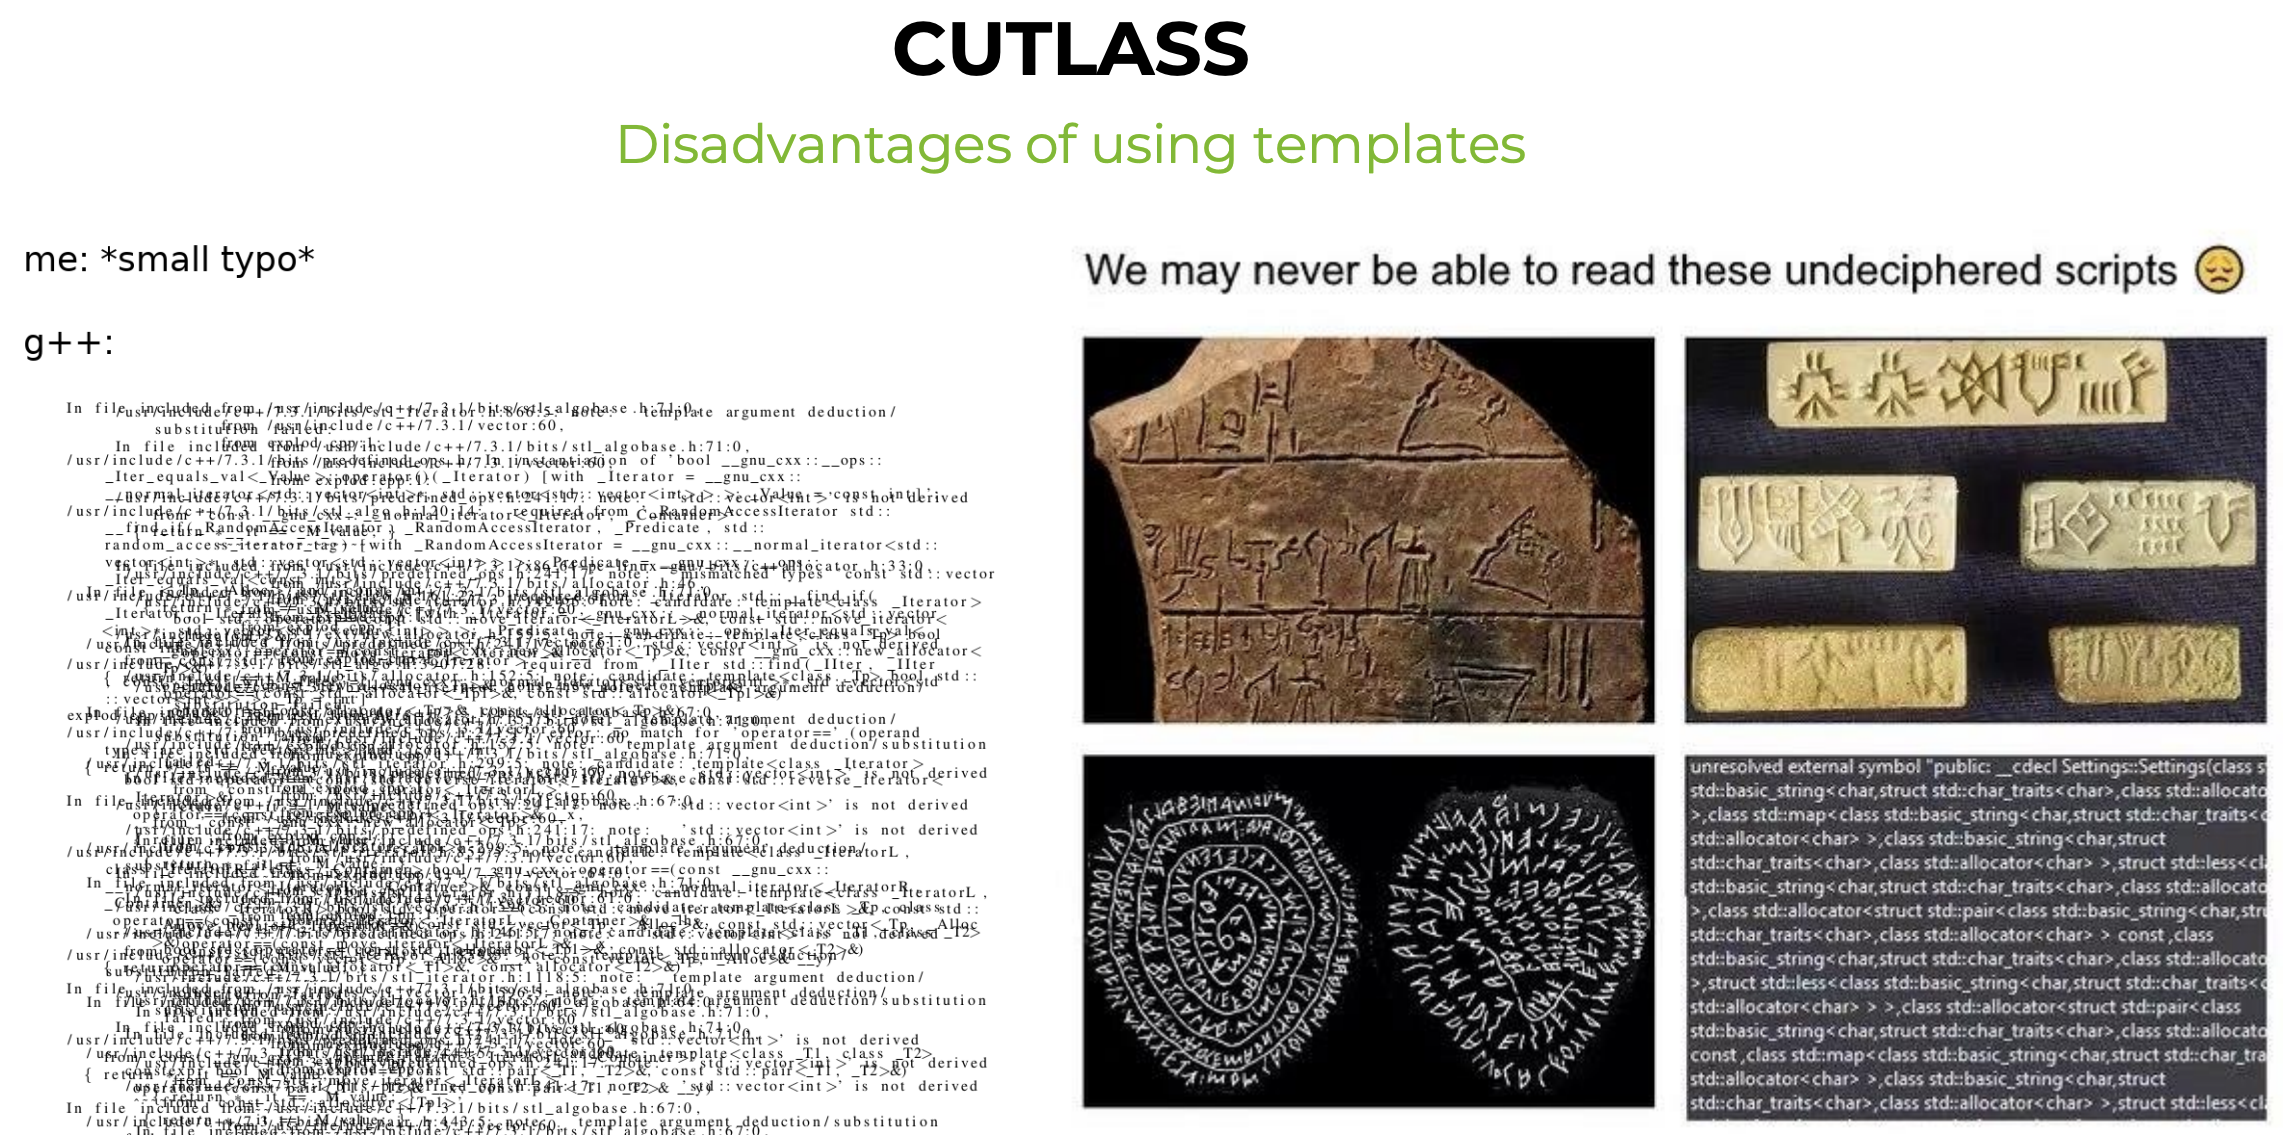
\includegraphics[width=0.8\textwidth]{day8_pm/img/2-templates}
		\caption{Cite: Yoolc's Sharing on CUTLASS}
	\end{figure}
\end{frame}

\subsection{Concurrency Support}
% 按时间引入 C++ 对并行编程的支持
% C++11:Threads, Mutual exclusion, Atomic operations, Condition variables, Futures
% C++20:Cooperative cancellation, Semaphores, Latches and Barriers
\begin{frame}[fragile]{Concurrency support library}
	\begin{itemize}
		\item \textbf{C++11} (We will learn):
		      \begin{itemize}
			      \item \texttt{<thread>}: Create and manage threads
			      \item \texttt{<mutex>}: Mutual exclusion for shared data
			      \item \texttt{<atomic>}: Atomic operations for thread safety
			      \item \texttt{<condition\_variable>}: Synchronization between threads
			      \item \texttt{<future>}: Asynchronous results
		      \end{itemize}
		\item \textbf{C++20}:
		      \begin{itemize}
			      \item \texttt{<stop\_token>}: Cooperative cancellation
			      \item \texttt{<semaphore>}, \texttt{<latch>}, and \texttt{<barrier>}: Advanced synchronization
		      \end{itemize}
	\end{itemize}
\end{frame}

\section{<thread>}

\subsection{Basic Thread Management}

\begin{frame}[fragile]{Launching a Thread}
	\textbf{C++ Thread Constructor:}
	\begin{minted}{cpp}
template< class F, class... Args >
    explicit thread( F&& f, Args&&... args );
thread( thread&& other ) noexcept; // Move constructor
    \end{minted}
	\begin{itemize}
		\item \texttt{other}: another thread object to construct this thread object with
		\item \texttt{f}: Callable object to execute in the new thread
		\item \texttt{args}: Arguments to pass to the new function
	\end{itemize}
\end{frame}

\begin{frame}[fragile]{Launching a Thread - Basic Examples}
	\begin{columns}
		\begin{column}{0.5\textwidth}
			\textbf{Simple Function}
			\begin{minted}{cpp}
#include <thread>
#include <iostream>

void hello() {
    cout << "Hello from thread!"
              << endl;
}

int main() {
    thread t(hello);
    t.join();
    return 0;
}
			\end{minted}
		\end{column}
		\begin{column}{0.5\textwidth}
			\textbf{Function with Parameters}
			\begin{minted}{cpp}
#include <thread>
#include <iostream>

void worker(int id, const string& name) {
    cout << "Worker " << id
              << " (" << name << ") running"
              << endl;
}

int main() {
    thread t(worker, 42, "Alice");
    t.join();
    return 0;
}
			\end{minted}
		\end{column}
	\end{columns}
\end{frame}

\begin{frame}[fragile]{Launching a Thread - Function Objects and Lambdas}
	\begin{columns}
		\begin{column}{0.5\textwidth}
			\textbf{Function Object}
			\begin{minted}{cpp}
#include <thread>
#include <iostream>

class background_task {
public:
    void operator()() {
        cout << "Background task running"
                  << endl;
    }
};

int main() {
    background_task task;
    thread t(task);
    t.join();
    return 0;
}
			\end{minted}
		\end{column}
		\begin{column}{0.5\textwidth}
			\textbf{Lambda Expression}
			\begin{minted}{cpp}
#include <thread>
#include <iostream>

int main() {
    thread t([]() {
        cout << "Lambda task running"
                  << endl;
    });

    t.join();
    return 0;
}
			\end{minted}
		\end{column}
	\end{columns}
\end{frame}

\begin{frame}[fragile]{\emoji{warning} Most Vexing Parse Problem}
	\textbf{Common Pitfall:} C++ interprets ambiguous syntax as function declarations

	\begin{minted}{cpp}
struct background_task {
    void operator()() {
        // do work
    }
};

// WRONG! This declares a function, not creates a thread!
thread my_thread(background_task());

// Correct ways:
thread t1{background_task()};    // uniform initialization
thread t2((background_task()));  // extra parentheses
thread t3(background_task{});    // temporary object
	\end{minted}

	\textbf{Recommended:} Use uniform initialization \texttt{\{\}} or lambdas to avoid parsing issues
\end{frame}

\begin{frame}[fragile]{Waiting for a Thread to Complete}
	\textbf{join():} Wait for thread completion before continuing

	\begin{columns}
		\begin{column}{0.5\textwidth}
			\begin{minted}{cpp}
void worker(int seconds) {
    this_thread::sleep_for(
        chrono::seconds(seconds));
    cout << "Work done!" << endl;
}
int main() {
    cout << "Starting thread..." << endl;
    thread t(worker, 2);
    cout << "Waiting for completion..."
              << endl;
    t.join();  // Block until thread finishes
    cout << "Thread completed!" << endl;
    return 0;
}
			\end{minted}
			\textbf{Basic join() Example}
		\end{column}
		\begin{column}{0.5\textwidth}
			\begin{minted}{cpp}
void worker(int id) {
    cout << "Worker " << id
              << " running" << endl;
}
int main() {
    vector<thread> threads;
    for(int i = 0; i < 4; i++) {
        threads.emplace_back(worker, i);
    }
    for(auto& t : threads) {
        t.join();
    }
    cout << "All threads completed!"
              << endl;
    return 0;
}
			\end{minted}
			\textbf{Multiple Threads}
		\end{column}
	\end{columns}
\end{frame}

\begin{frame}[fragile]{Waiting in Exceptional Circumstances}
	\textbf{Problem:} Exception-safe thread management with RAII

	\begin{columns}
		\begin{column}{0.4\textwidth}
			\begin{minted}{cpp}
void do_work() {
    thread t([]() {
        // long running task
    });

    // If exception thrown here,
    // t.join() won't be called!
    risky_operation();

    t.join();  // May not be reached
}
			\end{minted}
			\textbf{Without RAII - Dangerous!}
		\end{column}
		\begin{column}{0.6\textwidth}
			\begin{minted}{cpp}
class thread_guard {
    thread& t;
public:
    explicit thread_guard(thread& t_) : t(t_) {}
    ~thread_guard() { if(t.joinable()) { t.join(); } }
    thread_guard(const thread_guard&) = delete;
    thread_guard& operator=(const thread_guard&) = delete;
};
void do_work() {
    thread t([]() { /* long running task */ });
    thread_guard g(t);
    risky_operation();  // Safe!
    // Destructor ensures join()
}
			\end{minted}
			\textbf{With RAII - Safe!}
		\end{column}
	\end{columns}
\end{frame}

\begin{frame}[fragile]{Running Threads in the Background}
	\textbf{detach():} Run thread independently without waiting

	\begin{columns}
		\begin{column}{0.5\textwidth}
			\begin{minted}{cpp}
    thread t(background_task);
    // Detach - thread runs independently
    t.detach();

    cout << "Main continues..." << endl;
    // Main might end before background finishes!
    this_thread::sleep_for(
        chrono::seconds(3));
			\end{minted}
			\textbf{Detached Thread Example}
		\end{column}
		\begin{column}{0.5\textwidth}
			\begin{minted}{cpp}
thread t(worker);
// Check if thread can be joined
if (t.joinable()) {
    cout << "Thread is joinable" << endl;
    t.join();
}
// After join/detach, not joinable
cout << t.joinable() << endl;  // false
thread t2(worker);
t2.detach();
cout << t2.joinable() << endl;  // false
			\end{minted}
			\textbf{Checking Thread State}
		\end{column}
	\end{columns}

	%\scriptsize
	\textbf{Important:} Every thread must be either joined or detached before destruction!
\end{frame}

\subsection{Passing Arguments to a Thread Function}

\begin{frame}[fragile]{Parameter Passing Basics}
	\textbf{Key Principle:} Thread constructor copies arguments as rvalues

	\textbf{String Conversion Issues}
	\begin{columns}
		\begin{column}{0.6\textwidth}
			\begin{minted}{cpp}
void print_string(const string& str) {
    cout << str << endl;
}

// UNSAFE! Pointer passed, conversion happens in new thread
thread unsafe_executor() {
    char buffer[] = "Hello World";
    return thread(print_string, buffer);
}
// SAFE! Force conversion before thread creation
thread safe_executor() {
    char buffer[] = "Hello World";
    return thread(print_string, string(buffer));
}
			\end{minted}
		\end{column}
		\begin{column}{0.4\textwidth}
			\begin{minted}{cpp}
try {
    thread t1 = unsafe_executor();
    t1.join();
} catch (const exception& e) {
    cerr << "Error in unsafe_executor: " << e.what() << endl;
}
thread t2 = safe_executor();
t2.join();
			\end{minted}
		\end{column}
	\end{columns}
\end{frame}

\begin{frame}[fragile]{Advanced Parameter Passing}

	\textbf{Member Functions}
	\begin{minted}{cpp}
class X {
public:
    void do_work(int n) {
        cout << "Work " << n
                  << " done by object" << endl;
    }
};

int main() {
    X my_x;

    // Pass member function and object
    thread t(&X::do_work, &my_x, 42);

    t.join();
    return 0;
}
			\end{minted}
\end{frame}

\subsection{Transferring Ownership of a Thread}

\begin{frame}[fragile]{Move Semantics with Threads}
	\textbf{thread is move-only:} Cannot be copied, only moved

	\begin{columns}
		\begin{column}{0.5\textwidth}
			\begin{minted}{cpp}
thread t1(worker);
// Move constructor
thread t2 = move(t1);
// t1 is now empty

// Move from function
thread t3 = create_thread();

// t1.join();  // ERROR! t1 is empty
t2.join();
t3.join();
			\end{minted}
			\textbf{Basic Move Operations}
		\end{column}
		\begin{column}{0.5\textwidth}
			\begin{minted}{cpp}
thread t1(task1);
thread t2(task2);

// Join first thread
t1.join();

// Move assign - t1 takes over t2
t1 = move(t2);
// t2 is now empty

t1.join();
			\end{minted}
			\textbf{Move Assignment}
		\end{column}
	\end{columns}
\end{frame}

\begin{frame}[fragile]{Transferring Ownership with Move - Advanced}
	\textbf{Move Semantics:} Transfer unique resources to threads

	\begin{minted}{cpp}
void process_data(unique_ptr<int> ptr) {
    if (ptr) {
        cout << "Processing: " << *ptr << endl;
        *ptr *= 2;
        cout << "Result: " << *ptr << endl;
    }
}

int main() {
    auto ptr = make_unique<int>(42);

    // Transfer ownership to thread using move
    thread t(process_data, move(ptr));

    // ptr is now nullptr, ownership transferred
    assert(ptr == nullptr);

    t.join();
    return 0;
}
	\end{minted}
\end{frame}

\begin{frame}[fragile]{Thread Containers and RAII}
	\textbf{Managing Multiple Threads with Move Semantics}

	\begin{columns}
		\begin{column}{0.5\textwidth}
			\begin{minted}{cpp}
class scoped_thread {
    thread t;
public:
    explicit scoped_thread(thread t_) : t(move(t_)) {
        if (!t.joinable()) {
            throw logic_error("No thread");
        }
    }

    ~scoped_thread() {
        t.join();
    }

    scoped_thread(const scoped_thread&) = delete;
    scoped_thread& operator=(const scoped_thread&) = delete;
};
            \end{minted}
		\end{column}
		\begin{column}{0.5\textwidth}
			\begin{minted}{cpp}
int main() {
    vector<scoped_thread> threads;

    for (int i = 0; i < 3; ++i) {
        threads.emplace_back(thread(worker, i));
    }

    // Threads automatically joined when scoped_thread destructors run
    return 0;
}
	\end{minted}
		\end{column}
	\end{columns}
\end{frame}

\subsection{Choosing the Number of Threads at Runtime}

\begin{frame}[fragile]{Hardware Concurrency}
	\textbf{thread::hardware\_concurrency():} Get optimal thread count

	\begin{minted}{cpp}
unsigned int num_threads = thread::hardware_concurrency();

if (num_threads == 0) {
    num_threads = 2;  // Fallback if not available
}

cout << "Using " << num_threads << " threads" << endl;

vector<thread> threads;
for (unsigned int i = 0; i < num_threads; ++i) {
    threads.emplace_back(worker, i);
}

for (auto& t : threads) {
    t.join();
}
	\end{minted}
\end{frame}

\begin{frame}[fragile]{Parallel Accumulate - Helper Function}
	\textbf{Step 1:} Define the worker function for each thread

	\begin{minted}{cpp}
template<typename Iterator, typename T>
void accumulate_block(Iterator first, Iterator last, T& result) {
    result = accumulate(first, last, result);
}
	\end{minted}

	\textbf{Function Purpose:}
	\begin{itemize}
		\item Each thread processes a block of data
		\item Computes sum of elements from \texttt{first} to \texttt{last}
		\item Stores result in reference parameter
		\item Uses standard library \texttt{accumulate} function
	\end{itemize}

	\vspace{1em}
	\textbf{Next:} Calculate optimal thread configuration
\end{frame}

\begin{frame}[fragile]{Parallel Accumulate - Thread Configuration}
	\textbf{Step 2:} Calculate optimal number of threads and work distribution

	\begin{minted}{cpp}
template<typename Iterator, typename T>
T parallel_accumulate(Iterator first, Iterator last, T init) {
    unsigned long const length = distance(first, last);
    if (!length) return init;

    // Configuration parameters
    unsigned long const min_per_thread = 25;
    unsigned long const max_threads =
        (length + min_per_thread - 1) / min_per_thread;

    unsigned long const hardware_threads =
        thread::hardware_concurrency();

    unsigned long const num_threads =
        min(hardware_threads != 0 ? hardware_threads : 2, max_threads);

    unsigned long const block_size = length / num_threads;
    // ...
}
	\end{minted}

	\textbf{Logic:} Balance between overhead and parallelism
\end{frame}

\begin{frame}[fragile]{Parallel Accumulate - Thread Creation \& Execution}
	\textbf{Step 3:} Create threads and distribute work

	\begin{minted}{cpp}
// Storage for results and threads
vector<T> results(num_threads);
vector<thread> threads(num_threads - 1);
// Create worker threads (all but last)
Iterator block_start = first;
for (unsigned long i = 0; i < (num_threads - 1); ++i) {
    Iterator block_end = block_start;
    advance(block_end, block_size);
    threads[i] = thread(accumulate_block<Iterator, T>,
                        block_start, block_end, ref(results[i]));
    block_start = block_end;
}
// Main thread handles the last block
accumulate_block(block_start, last, results[num_threads - 1]);
// Wait for all threads and combine results
for (auto& entry : threads) entry.join();
return accumulate(results.begin(), results.end(), init);
	\end{minted}
\end{frame}

\subsection{Identifying Threads}

\begin{frame}[fragile]{Thread IDs - Basic Usage}
	\textbf{thread::id:} Unique identifier for each thread

	\begin{minted}{cpp}
void worker() {
    cout << "Thread ID: " << this_thread::get_id() << endl;
}
cout << "Main thread ID: " << this_thread::get_id() << endl;
thread t(worker);
cout << "Worker thread ID: " << t.get_id() << endl;
t.join();
cout << "After join: " << t.get_id() << endl;  // Default ID
	\end{minted}

	\textbf{Key Functions:}
	\begin{itemize}
		\item \texttt{this\_thread::get\_id()}: Get current thread's ID
		\item \texttt{thread\_obj.get\_id()}: Get thread object's ID
		\item Default-constructed ID represents "no thread"
	\end{itemize}
\end{frame}

\begin{frame}[fragile]{Thread ID Properties \& Usage}
	\textbf{Thread ID Characteristics:}
	\begin{itemize}
		\item \textbf{Unique:} Each executing thread has a unique ID
		\item \textbf{Comparable:} Can be compared for equality and ordering
		\item \textbf{Hashable:} Can be used as keys in containers
		\item \textbf{Default-constructible:} Default ID represents "no thread"
	\end{itemize}

	\begin{minted}{cpp}
// Thread ID comparison
thread::id main_id = this_thread::get_id();
thread::id default_id;  // Default-constructed
cout << "IDs equal: " << (main_id == default_id) << endl;  // false
// Use as container key
unordered_set<thread::id> thread_set;
thread_set.insert(main_id);
// Useful for debugging and thread identification
map<thread::id, string> thread_names;
thread_names[this_thread::get_id()] = "main_thread";
	\end{minted}
\end{frame}

\begin{frame}[fragile]{\emoji{light-bulb} Best Practices Summary}
	\scriptsize
	\textbf{Thread Management:}
	\begin{itemize}
		\item Always \texttt{join()} or \texttt{detach()} threads before destruction
		\item Use RAII (e.g., \texttt{thread\_guard}) for exception safety
		\item Prefer \texttt{move} semantics for thread ownership transfer
	\end{itemize}

	\textbf{Parameter Passing:}
	\begin{itemize}
		\item Be careful with string literals - convert to \texttt{std::string} explicitly
		\item Use \texttt{std::ref()} for reference parameters
		\item Move unique resources (e.g., \texttt{unique\_ptr}) when transferring ownership
	\end{itemize}

	\textbf{Performance:}
	\begin{itemize}
		\item Use \texttt{hardware\_concurrency()} to determine optimal thread count
		\item Balance thread overhead vs. parallelism (minimum work per thread)
		\item Consider thread pool patterns for repeated tasks
	\end{itemize}
\end{frame}

\begin{frame}[fragile]{\emoji{books} Key Takeaways}
	\textbf{Core Concepts Mastered:}
	\begin{enumerate}
		\item \textbf{Thread Creation:} Functions, lambdas, member functions
		\item \textbf{Synchronization:} \texttt{join()} vs \texttt{detach()} patterns
		\item \textbf{Exception Safety:} RAII wrappers for automatic cleanup
		\item \textbf{Move Semantics:} Efficient thread and resource transfer
		\item \textbf{Runtime Optimization:} Hardware-aware thread configuration
	\end{enumerate}

	\vspace{1em}
	\textbf{Next Steps:}
	\begin{itemize}
		\item Thread synchronization with mutexes and locks
		\item Condition variables for thread coordination
		\item Parallel algorithms in the standard library
	\end{itemize}

	\vspace{1em}
	\textbf{Remember:} Modern C++ threading is about safety, efficiency, and expressiveness!
\end{frame}

\section{<mutex>}

\subsection{Race Conditions}
\begin{frame}[fragile]{Race Condition Problem}
	\textbf{The Core Issue}: Multiple threads accessing shared data

	\begin{minted}{cpp}
int counter = 0;  // Shared variable

void increment_unsafe(int iterations) {
    for(int i = 0; i < iterations; i++) {
        counter++;  // NOT thread-safe!
    }
}
	\end{minted}

	\begin{minted}{cpp}
// 4 threads, each incrementing 100000 times
std::vector<std::thread> threads;
for(int i = 0; i < 4; i++) {
    threads.emplace_back(increment_unsafe, 100000);
}
for(auto& t : threads) { t.join(); }

// Expected: 400000, Actual: varies (e.g., 387234)
	\end{minted}
\end{frame}

\begin{frame}[fragile]{Why Race Conditions Happen}
	\textbf{Assembly breakdown of} \texttt{counter++}:

	\begin{columns}
		\begin{column}{0.4\textwidth}
			\begin{minted}{asm}
mov eax, [counter]  // Read
add eax, 1          // Modify
mov [counter], eax  // Write
			\end{minted}
		\end{column}
		\begin{column}{0.6\textwidth}
			\textbf{Thread Interleaving Problem}:
			\begin{itemize}
				\item Thread 1 reads counter = 0
				\item Thread 2 reads counter = 0
				\item Thread 1 writes counter = 1
				\item Thread 2 writes counter = 1
				\item \textbf{Lost update!} Should be 2
			\end{itemize}
		\end{column}
	\end{columns}

	\vspace{0.5em}
	\textbf{Critical Section}: Code accessing shared resources
\end{frame}

\subsection{Protecting Shared Data with Mutexes}
\begin{frame}[fragile]{C++ Mutex Solution}
	\textbf{Using} \texttt{std::mutex} \textbf{with RAII}:

	\begin{minted}{cpp}
std::mutex counter_mutex;
int counter = 0;

void increment_safe(int iterations) {
    for(int i = 0; i < iterations; i++) {
        std::lock_guard<std::mutex> lock(counter_mutex);
        counter++;  // Now thread-safe!
        // Automatic unlock when lock goes out of scope
    }
}
	\end{minted}

	\textbf{RAII Benefits}:
	\begin{itemize}
		\item Exception safety
		\item Automatic cleanup
		\item No manual lock/unlock
	\end{itemize}
\end{frame}

\begin{frame}[fragile]{Structured Data Protection}
	\textbf{Class-based Protection}:

	\begin{minted}{cpp}
class ThreadSafeCounter {
private:
    int count = 0;
    mutable std::mutex mtx;

public:
    void increment() {
        std::lock_guard<std::mutex> lock(mtx);
        ++count;
    }

    int get() const {
        std::lock_guard<std::mutex> lock(mtx);
        return count;
    }
};
	\end{minted}

	\textbf{Key Principle}: Keep data and mutex together
\end{frame}

\subsection{Deadlock Prevention}
\begin{frame}[fragile]{The Deadlock Problem}
	\textbf{Classic Deadlock Scenario}:

	\begin{minted}{cpp}
std::mutex mutex1, mutex2;

void thread1() {
    std::lock_guard<std::mutex> lock1(mutex1);
    // ... some work ...
    std::lock_guard<std::mutex> lock2(mutex2);  // Waits forever
}

void thread2() {
    std::lock_guard<std::mutex> lock2(mutex2);
    // ... some work ...
    std::lock_guard<std::mutex> lock1(mutex1);  // Waits forever
}
	\end{minted}

	\textbf{Result}: Circular wait → Deadlock!
\end{frame}

\begin{frame}[fragile]{Deadlock Solutions}
	\textbf{Strategy 1: Ordered Locking}
	\begin{minted}{cpp}
// Always lock in same order
std::lock_guard<std::mutex> lock1(mutex1);  // First
std::lock_guard<std::mutex> lock2(mutex2);  // Second
	\end{minted}

	\textbf{Strategy 2: Atomic Multi-lock}
	\begin{minted}{cpp}
std::unique_lock<std::mutex> lock1(mutex1, std::defer_lock);
std::unique_lock<std::mutex> lock2(mutex2, std::defer_lock);
std::lock(lock1, lock2);  // Atomic acquisition
	\end{minted}
\end{frame}

\begin{frame}[fragile]{Deadlock Solutions}
	\textbf{Strategy 3: Address-based Ordering}
	\begin{minted}{cpp}
if (&mutex1 < &mutex2) {
    std::lock_guard<std::mutex> lock1(mutex1);
    std::lock_guard<std::mutex> lock2(mutex2);
} else {
    std::lock_guard<std::mutex> lock2(mutex2);
    std::lock_guard<std::mutex> lock1(mutex1);
}
	\end{minted}
\end{frame}

\begin{frame}[fragile]{Practical Example: Bank Transfer}
	\begin{minted}{cpp}
class BankAccount {
    double balance;
    mutable std::mutex mtx;
public:
    static void transfer(BankAccount& from, BankAccount& to,
                        double amount) {
        // Prevent deadlock with consistent ordering
        if (&from < &to) {
            std::lock_guard<std::mutex> lock1(from.mtx);
            std::lock_guard<std::mutex> lock2(to.mtx);
        } else {
            std::lock_guard<std::mutex> lock1(to.mtx);
            std::lock_guard<std::mutex> lock2(from.mtx);
        }
        from.balance -= amount;
        to.balance += amount;
    }
};
	\end{minted}
\end{frame}

\subsection{Key Takeaways}
\begin{frame}{Mutex Best Practices}
	\begin{enumerate}
		\item \textbf{Use RAII}: \texttt{std::lock\_guard} over manual lock/unlock
		\item \textbf{Keep critical sections short}: Minimize lock duration
		\item \textbf{Consistent lock ordering}: Prevent deadlocks
		\item \textbf{Encapsulate}: Keep data and mutex together
		\item \textbf{Avoid nested locks}: When possible
	\end{enumerate}
\end{frame}

\begin{frame}{C++ Mutex Tools}
	\begin{itemize}
		\item \texttt{std::mutex} - Basic mutual exclusion
		\item \texttt{std::lock\_guard} - RAII lock wrapper
		\item \texttt{std::unique\_lock} - Flexible locking
		\item \texttt{std::lock()} - Multi-mutex atomic locking
	\end{itemize}
\end{frame}

\section{<condition\_variable>}

\subsection{Waiting for an Event or Other Condition}
\begin{frame}[fragile]{The Problem with Polling}
	\textbf{Inefficient Waiting with} \texttt{sleep\_for}:

	\begin{minted}{cpp}
bool data_ready = false;
std::mutex data_mutex;

void consumer() {
    while (true) {
        {
            std::lock_guard<std::mutex> lock(data_mutex);
            if (data_ready) {  /* Process data */
                data_ready = false; break;
            }
        }
        std::this_thread::sleep_for(std::chrono::milliseconds(100));
        // Wastes CPU cycles and introduces latency!
    }
}
	\end{minted}

	\begin{itemize}
		\item CPU wastage from constant polling
		\item Unnecessary latency, unpredictable timing
	\end{itemize}
\end{frame}

\begin{frame}[fragile]{Event-Driven Solution}
	\textbf{Better Approach}: Wait for notification instead of polling

	\begin{minted}{cpp}
std::mutex m;
std::condition_variable cv;
bool data_ready = false;
void producer() { /* Prepare data...*/
    {
        std::lock_guard<std::mutex> lock(m);
        data_ready = true;
    }
    cv.notify_one();  // Wake up waiting thread
}

void consumer() {
    std::unique_lock<std::mutex> lock(m);
    cv.wait(lock, []{return data_ready;});
    // Data is ready, process it
}
	\end{minted}

	\textbf{Benefits}: Efficient waiting, immediate response, no CPU waste
\end{frame}

\subsection{Waiting for a Condition with Condition Variables}
\begin{frame}[fragile]{Condition Variable Types}
	\textbf{Two Implementations Available}:

	\begin{itemize}
		\item \texttt{std::condition\_variable}: Works only with \texttt{std::mutex}
		\item \texttt{std::condition\_variable\_any}: Works with any mutex type (extra overhead)
	\end{itemize}
\end{frame}

\begin{frame}[fragile]{Condition Variable Basics}
	\begin{minted}{cpp}
std::mutex m;
std::condition_variable cv;
bool condition = false;

void waiter() {
    std::unique_lock<std::mutex> lock(m);
    cv.wait(lock, []{return condition;});
    // Condition is now true
}

void notifier() {
    {
        std::lock_guard<std::mutex> lock(m);
        condition = true;
    }
    cv.notify_one();  // or notify_all()
}
	\end{minted}
\end{frame}

\begin{frame}[fragile]{Understanding wait() Overloads}
	\textbf{Two versions of} \texttt{wait()}:

	\begin{minted}{cpp}
// Version 1: Basic wait
void wait(std::unique_lock<std::mutex>& lock);

// Version 2: Wait with predicate (recommended)
template<class Predicate>
void wait(std::unique_lock<std::mutex>& lock, Predicate pred);
	\end{minted}

	\textbf{Predicate version equivalent to}:
	\begin{minted}{cpp}
while (!pred()) wait(lock);  // Handles spurious wakeups
	\end{minted}
\end{frame}


\begin{frame}[fragile]{How wait() Works Internally}
	\begin{enumerate}
		\item Atomically releases the mutex
		\item Blocks current thread
		\item Waits for notification
		\item Re-acquires mutex when awakened
		\item Checks predicate (if provided)
	\end{enumerate}
\end{frame}

\begin{frame}[fragile]{Why unique\_lock Instead of lock\_guard?}
	\textbf{Condition variables need flexible locking}:

	\begin{minted}{cpp}
// This WON'T work - lock_guard can't be unlocked
std::lock_guard<std::mutex> lock(m);
cv.wait(lock);  // Compiler error!

// This WORKS - unique_lock supports unlock/relock
std::unique_lock<std::mutex> lock(m);
cv.wait(lock);  // Can unlock and relock automatically
	\end{minted}

	\vspace{0.5em}
	\textbf{Key Difference}:
	\begin{itemize}
		\item \texttt{lock\_guard}: RAII-only, cannot be manually unlocked
		\item \texttt{unique\_lock}: Flexible, supports deferred/conditional locking
	\end{itemize}
\end{frame}

\begin{frame}[fragile]{Notification Methods}
	\textbf{Two ways to notify waiting threads}:

	\begin{minted}{cpp}
std::condition_variable cv;

// Wake up ONE waiting thread
cv.notify_one();

// Wake up ALL waiting threads
cv.notify_all();
	\end{minted}

	\vspace{1em}
	\textbf{When to use each}:
	\begin{itemize}
		\item \texttt{notify\_one()}: When only one thread should process the event
		\item \texttt{notify\_all()}: When multiple threads need to check the condition
	\end{itemize}

	\vspace{0.5em}
	\textbf{Best Practice}: Always modify shared state before notifying
	\begin{minted}{cpp}
{
    std::lock_guard<std::mutex> lock(m);
    ready = true;  // Change state first
}
cv.notify_one();   // Then notify
	\end{minted}
\end{frame}

\subsection{Building a Thread-Safe Queue with Condition Variables}
\begin{frame}[fragile]{Thread-Safe Queue Design}
	\textbf{Requirements}:
	\begin{itemize}
		\item Multiple producers can push safely
		\item Multiple consumers can pop safely
		\item Consumers wait when queue is empty
		\item No busy waiting or polling
	\end{itemize}
\end{frame}

\begin{frame}[fragile]{Thread-Safe Queue Design}
	\textbf{Core Components}:
	\begin{minted}{cpp}
template<typename T>
class ThreadSafeQueue {
private:
    std::queue<T> queue_;
    mutable std::mutex mutex_;
    std::condition_variable condition_;

public:
    void push(const T& item);
    T pop();
    bool empty() const;
    size_t size() const;
};
	\end{minted}
\end{frame}

\begin{frame}[fragile]{Implementation: Push Operation}
	\textbf{Producer side - Adding items}:

	\begin{minted}{cpp}
template<typename T>
void ThreadSafeQueue<T>::push(const T& item) {
    {   std::lock_guard<std::mutex> lock(mutex_);
        queue_.push(item); }
    condition_.notify_one();  // Wake up waiting consumer
}
template<typename T>
void ThreadSafeQueue<T>::push(T&& item) {
    {   std::lock_guard<std::mutex> lock(mutex_);
        queue_.push(std::move(item)); }
    condition_.notify_one();
}
	\end{minted}

	\textbf{Key Points}:
	\begin{itemize}
		\item Lock only while modifying queue
		\item Notify after releasing lock
		\item Support both copy and move semantics
	\end{itemize}
\end{frame}

\begin{frame}[fragile]{Implementation: Pop Operation}
	\textbf{Consumer side - Retrieving items}:

	\begin{minted}{cpp}
template<typename T>
T ThreadSafeQueue<T>::pop() {
    std::unique_lock<std::mutex> lock(mutex_);

    // Wait until queue is not empty
    condition_.wait(lock, [this] {
        return !queue_.empty();
    });

    T item = std::move(queue_.front());
    queue_.pop();
    return item;
}
	\end{minted}
\end{frame}


\begin{frame}[fragile]{Implementation: Pop Operation}
	\textbf{Alternative with timeout}:
	\begin{minted}{cpp}
template<typename T>
bool ThreadSafeQueue<T>::try_pop(T& item,
                                 std::chrono::milliseconds timeout) {
    std::unique_lock<std::mutex> lock(mutex_);
    if (condition_.wait_for(lock, timeout,
                           [this] { return !queue_.empty(); })) {
        item = std::move(queue_.front());
        queue_.pop();
        return true;
    }
    return false;  // Timeout occurred
}
	\end{minted}
\end{frame}

\begin{frame}[fragile]{Complete Usage Example}
	\textbf{Producer-Consumer with Thread-Safe Queue}:

	\begin{minted}{cpp}
ThreadSafeQueue<int> queue;
void producer(int start, int count) {
    for (int i = start; i < start + count; ++i) {
        queue.push(i);
        std::this_thread::sleep_for(std::chrono::milliseconds(10));
    }
}
void consumer(int id) {
    for (int i = 0; i < 5; ++i) {
        int value = queue.pop();  // Blocks until item available
        std::cout << "Consumer " << id << " got: " << value << std::endl;
    }
}
int main() {
    std::thread prod1(producer, 0, 10);
    std::thread cons1(consumer, 1);
    std::thread cons2(consumer, 2);
    prod1.join(); cons1.join(); cons2.join();
    return 0;
}
	\end{minted}
\end{frame}

\subsection{Key Takeaways}
\begin{frame}{Condition Variable Best Practices}
	\textbf{Essential Guidelines}:
	\begin{enumerate}
		\item \textbf{Always use predicates}: Protects against spurious wakeups
		\item \textbf{Use unique\_lock}: Required for condition variable flexibility
		\item \textbf{Modify state before notify}: Ensure consistency
		\item \textbf{Keep critical sections short}: Minimize lock contention
		\item \textbf{Choose notify method wisely}: \texttt{notify\_one()} vs \texttt{notify\_all()}
	\end{enumerate}
\end{frame}

\begin{frame}{Condition Variable Best Practices}
	\textbf{Common Patterns}:
	\begin{itemize}
		\item Producer-Consumer queues
		\item Event signaling
		\item Worker thread pools
		\item Barrier synchronization
	\end{itemize}

	\vspace{1em}
	\textbf{Remember}: Condition variables are more efficient than polling for event-driven synchronization!
\end{frame}

\section{Parallel Algorithms}

\subsection{Parallelizing the Standard Library Algorithms}
\begin{frame}[fragile]{C++17 Parallel Algorithms}
	\textbf{Enhancement to STL Algorithms}: Parallel execution support

	\begin{minted}{cpp}
#include <execution>

std::vector<int> my_data = {3, 1, 4, 1, 5, 9, 2, 6};

// Serial execution (C++11/14)
std::sort(my_data.begin(), my_data.end());

// Parallel execution (C++17)
std::sort(std::execution::par, my_data.begin(), my_data.end());
	\end{minted}

	\textbf{Key Change}: Additional first parameter for execution policy

	\vspace{0.5em}
	\textbf{Available for}: \texttt{std::sort}, \texttt{std::for\_each}, \texttt{std::transform}, \texttt{std::reduce}, and many more!
\end{frame}

\begin{frame}[fragile]{Similarity to OpenMP}
	\begin{minted}[fontsize=\scriptsize]{cpp}
#pragma omp parallel for
for(unsigned i=0;i<my_data.size();++i)
{
    do_stuff(my_data[i]);
}

std::for_each(std::execution::par, my_data.begin(), my_data.end(), do_stuff);
    \end{minted}
\end{frame}

\subsection{Execution Policies}
\begin{frame}[fragile]{Execution Policy Types}
	\textbf{Four execution policies available}:

	\begin{minted}{cpp}
// 1. Sequential (same as no policy)
std::execution::sequenced_policy      // std::execution::seq
// 2. Parallel
std::execution::parallel_policy       // std::execution::par
// 3. Parallel + Vectorized
std::execution::parallel_unsequenced_policy  // std::execution::par_unseq
// 4. Unsequenced (C++20)
std::execution::unsequenced_policy    // std::execution::unseq
std::sort(std::execution::seq, v.begin(), v.end());
std::sort(std::execution::par, v.begin(), v.end());
std::sort(std::execution::par_unseq, v.begin(), v.end());
	\end{minted}

	Execution policies is a \textbf{permission}, not a \textbf{requirement}.
\end{frame}

\begin{frame}{General Effects of Execution Policies}
	\textbf{std::execution::sequenced\_policy}:
	\begin{itemize}
		\item Same as traditional serial execution
		\item Single thread, sequential order
	\end{itemize}

	\textbf{std::execution::parallel\_policy}:
	\begin{itemize}
		\item Multiple threads allowed
		\item Operations may be interleaved
		\item No vectorization guarantees
	\end{itemize}
\end{frame}

\begin{frame}{General Effects of Execution Policies}

	\textbf{std::execution::parallel\_unsequenced\_policy}:
	\begin{itemize}
		\item Multiple threads + vectorization
		\item Operations may execute in any order
		\item Best performance potential
		\item Requires thread-safe operations
	\end{itemize}
\end{frame}

\setminted{
	fontsize=\scriptsize
}
\subsection{The Parallel Algorithms from the C++ Standard Library}
\begin{frame}[fragile]{Examples of Using Parallel Algorithms}
	\textbf{Parallel Transform}:
	\begin{minted}{cpp}
std::vector<int> input = {1, 2, 3, 4, 5};
std::vector<int> output(input.size());

std::transform(std::execution::par,
               input.begin(), input.end(),
               output.begin(),
               [](int x) { return x * x; });
	\end{minted}
\end{frame}

\begin{frame}[fragile]{Examples of Using Parallel Algorithms}
	\textbf{Parallel For Each}:
	\begin{minted}{cpp}
std::vector<std::string> words = {"hello", "world", "parallel"};

std::for_each(std::execution::par,
              words.begin(), words.end(),
              [](std::string& word) {
                  std::transform(word.begin(), word.end(),
                                word.begin(), ::toupper);
              });
	\end{minted}
\end{frame}

\begin{frame}[fragile]{Examples of Using Parallel Algorithms}
	\textbf{Parallel Reduction}:
	\begin{minted}{cpp}
std::vector<int> numbers(1000000);
std::iota(numbers.begin(), numbers.end(), 1);

// Parallel sum
auto sum = std::reduce(std::execution::par,
                       numbers.begin(), numbers.end(),
                       0);

// Parallel sum with custom operation
auto product = std::reduce(std::execution::par,
                          numbers.begin(), numbers.end(),
                          1,
                          std::multiplies<int>());
	\end{minted}
\end{frame}

\begin{frame}[fragile]{Examples of Using Parallel Algorithms}
	\textbf{Transform Reduce}:
	\begin{minted}{cpp}
auto squared_sum = std::transform_reduce(
    std::execution::par,
    numbers.begin(), numbers.end(),
    0,
    std::plus<>(),
    [](int x) { return x * x; }
);
	\end{minted}
\end{frame}

\setminted{
	fontsize=\tiny
}

\begin{frame}[fragile]{Counting Visits Example}
	\textbf{Website Analytics - Parallel Processing}:

	\begin{columns}
		\begin{column}{0.5\textwidth}
			\begin{minted}{cpp}
struct Visit {
    std::string page;
    int user_id;
    std::chrono::time_point<std::chrono::system_clock> timestamp;
};

std::vector<Visit> visits = load_visits();

// Count unique pages visited in parallel
std::sort(std::execution::par, visits.begin(), visits.end(),
          [](const Visit& a, const Visit& b) {
              return a.page < b.page;
          });
    \end{minted}
		\end{column}
		\begin{column}{0.5\textwidth}
			\begin{minted}{cpp}
// Count visits per page
std::map<std::string, int> page_counts;
auto current = visits.begin();
while (current != visits.end()) {
    auto range_end = std::upper_bound(
        std::execution::par,
        current, visits.end(), *current,
        [](const Visit& a, const Visit& b) {
            return a.page < b.page;
        });

    page_counts[current->page] =
        std::distance(current, range_end);
    current = range_end;
}
            \end{minted}
		\end{column}
	\end{columns}
\end{frame}

\begin{frame}[fragile]{Performance Considerations}
	\textbf{When to Use Parallel Algorithms}:
	\begin{itemize}
		\item Large datasets (typically > 10,000 elements)
		\item CPU-intensive operations
		\item Independent computations
	\end{itemize}

	\textbf{Overhead Example}:
	\begin{minted}{cpp}
// Small dataset - sequential might be faster
std::vector<int> small_data(100);
std::sort(std::execution::seq, small_data.begin(), small_data.end());

// Large dataset - parallel beneficial
std::vector<int> large_data(1000000);
std::sort(std::execution::par, large_data.begin(), large_data.end());
	\end{minted}
\end{frame}

\begin{frame}{Thread Safety in Parallel Algorithms}
	\textbf{Thread Safety Requirements}:
	\begin{itemize}
		\item Operations must be thread-safe for \texttt{par} and \texttt{par\_unseq}
		\item Avoid shared mutable state
		\item Use atomic operations when necessary
	\end{itemize}
\end{frame}

\subsection{Assignment: GPU Execution with NVIDIA}
\begin{frame}{Homework Assignment}
	\textbf{Research Task}:
	\begin{enumerate}
		\item Review NVIDIA compiler manual (nvc++)
		\item Study how to run C++ standard algorithms on GPU
		\item Observe CUDA calls generated by the compiler
	\end{enumerate}

	\textbf{Experiment Steps}:
	\begin{enumerate}
		\item Load NVIDIA HPC SDK
		\item Compile parallel algorithms with GPU support
		\item Use correct compile option
		\item Analyze generated CUDA code
	\end{enumerate}
\end{frame}

\begin{frame}{Homework Assignment}
	\textbf{Expected Results}:
	\begin{itemize}
		\item Standard C++ code runs without modification
		\item GPU kernel functions are auto-generated
		\item \textcolor{gray}{Significant performance improvement observed}
	\end{itemize}

	\vspace{0.5em}
	\textbf{Tip}: Use \texttt{nvprof} or \texttt{nsys} for performance analysis
\end{frame}

\begin{frame}[fragile]{Assignment Example Code}
	\textbf{Compile Command}: \verb|nvc++ <correct_option> -O3 test.cpp -o test|
	\textbf{Test Code Template}:

	\begin{minted}{cpp}
const size_t N = 10'000'000;
std::vector<int> data(N);
std::iota(data.begin(), data.end(), 1);
std::random_shuffle(data.begin(), data.end());

auto start = std::chrono::high_resolution_clock::now();

// This should run on GPU with nvc++ and correct options
std::sort(std::execution::par_unseq,
            data.begin(), data.end());

auto end = std::chrono::high_resolution_clock::now();
auto duration = std::chrono::duration_cast<
    std::chrono::milliseconds>(end - start);

std::cout << "Sorting took: " << duration.count()
            << " ms" << std::endl;
    \end{minted}

\end{frame}

\section{Summary}

\begin{frame}{C++ Language Essentials}
	\begin{itemize}
		\item \textbf{Object-Oriented Programming:} Classes, inheritance, polymorphism
		\item \textbf{RAII (Resource Acquisition Is Initialization):} Automatic resource management
		\item \textbf{Move Semantics:} Efficient resource transfer with move constructors and assignment
		\item \textbf{Smart Pointers:} \texttt{unique\_ptr}, \texttt{shared\_ptr} for memory safety
		\item \textbf{Modern C++ Features:} Auto type deduction, range-based for loops, lambdas
		\item \textbf{Standard Template Library (STL):} Containers, algorithms, iterators
	\end{itemize}
\end{frame}

\begin{frame}{C++ Concurrency Pillars}
	\begin{itemize}
		\item \textbf{Thread Management:} Creating, joining, and detaching threads
		\item \textbf{Mutual Exclusion:} \texttt{std::mutex}, \texttt{std::lock\_guard}, \texttt{std::unique\_lock}
		\item \textbf{Thread Communication:} \texttt{std::condition\_variable} for signaling
		\item \textbf{Parallel Algorithms:} STL algorithms with execution policies
		\item \textcolor{gray}{\textbf{Atomic Operations:} Lock-free programming with \texttt{std::atomic}}
		\item \textcolor{gray}{\textbf{Memory Ordering:} Understanding memory consistency models}
	\end{itemize}
\end{frame}

\begin{frame}{Best Practices for Thread Management}
	\begin{itemize}
		\item \textbf{RAII for Locks:} Always use lock guards, avoid manual lock/unlock
		\item \textbf{Minimize Shared State:} Reduce data sharing between threads
		\item \textbf{Prefer Higher-Level Abstractions:} Use parallel algorithms over raw threads
		\item \textbf{Avoid Deadlocks:} Consistent lock ordering, timeout mechanisms
		\item \textbf{Exception Safety:} Ensure proper cleanup in exception scenarios
		\item \textbf{Thread-Local Storage:} Use for thread-specific data
	\end{itemize}
\end{frame}

\begin{frame}{Framework Comparison: OpenMP vs C++ Threads vs MPI}
	\begin{table}[h]
		\centering
		\footnotesize
		\begin{tabular}{|l|c|c|c|}
			\hline
			\textbf{Aspect}      & \textbf{OpenMP} & \textbf{C++ Threads} & \textbf{MPI}  \\
			\hline
			Learning Curve       & Low             & Medium               & High          \\
			\hline
			Development Time     & Fast            & Medium               & Slow          \\
			\hline
			Fine-grained Control & Limited         & High                 & High          \\
			\hline
			Memory Model         & Shared          & Shared               & Distributed   \\
			\hline
			Scalability          & Node-level      & Node-level           & Cluster-level \\
			\hline
			Debugging            & Easy            & Medium               & Hard          \\
			\hline
		\end{tabular}
	\end{table}
\end{frame}

\begin{frame}{When to Choose Which Framework}
	\begin{itemize}
		\item \textbf{OpenMP:}
		      \begin{itemize}
			      \item Quick parallelization of existing code
			      \item Loop-based parallelism
			      \item Prototyping and simple parallel tasks
		      \end{itemize}
		\item \textbf{C++ Threads:}
		      \begin{itemize}
			      \item Complex synchronization requirements
			      \item Object-oriented concurrent design
			      \item Integration with modern C++ features
		      \end{itemize}
		\item \textbf{MPI:}
		      \begin{itemize}
			      \item Distributed computing across multiple nodes
			      \item Large-scale scientific computing
			      \item Heterogeneous computing environments
		      \end{itemize}
	\end{itemize}
\end{frame}

\begin{frame}{Key Takeaways}
	\begin{itemize}
		\item \textbf{Concurrency is Complex:} Start simple, understand fundamentals first
		\item \textbf{Choose the Right Tool:} Match the framework to your problem domain
		\item \textbf{Safety First:} Use RAII, smart pointers, and high-level abstractions
		\item \textbf{Performance Matters:} Profile and measure, don't guess
		\item \textbf{Modern C++ Advantage:} Combines performance with safety and expressiveness
	\end{itemize}
\end{frame}

\begin{frame}{Next Steps for Further Study}
	\begin{itemize}
		\item \textbf{Advanced Topics:} Lock-free programming, memory models, coroutines
		\item \textbf{Libraries:} Intel TBB, Boost.Thread, OpenCL for GPU computing
		\item \textbf{Design Patterns:} Producer-consumer, thread pools, actor models
		\item \textbf{Performance Analysis:} Profiling tools, bottleneck identification
		\item \textbf{Real-world Projects:} Apply concepts to practical problems
	\end{itemize}
\end{frame}



% Q&A
\begin{frame}[standout]
	\Huge\textsc{Thank You}

	\vfill

	\LARGE\textsc{Any Questions?}
\end{frame}

\end{document}
